The studies of the \monohbb channel presented here are based on Monte Carlo simulations with version 2.4.3 of MadGraph 5 \cite{Alwall:2014hca} using a 
Universal FeynRules Output \cite{Degrande:2011ua} implementation of the 2HDM with Dark Matter mediator with a Yukawa sector of type II provided by the authors of \cite{Bauer:2017ota}.
The PDF set used for these simulations is the NNPDF  collaboration's NNPDF30\_lo\_as\_0130 PDF set,
 a leading order five-flavor (assuming massless $b$-quarks) PDF set with $\alpha_{S}(m_{Z}) = 0.130$ \cite{Ball:2014uwa}.
For the matrix element calculation in MG5, the five-flavor scheme is chosen, and the b-quark mass set to zero.

The matrix element generated for the parton-level studies is $ g g \rightarrow h  \chi \bar{\chi}$. %ref to feynmangraph, else cite Bauer:2017ota
For the $\ma-\tanb$ scan (\autoref{fig:monoHbb_tanb_scan_met}, \autoref{fig:monoHbb_sensi_full_ma_tanb}), 
the matrix element $b \bar{b} \rightarrow h  \chi \bar{\chi}$ is also generated.
The additional matrix element is generated because at high $\tanb$ and for a Yukawa sector of type II,
the $b \bar{b}$ initiated process can have an amplitude as large as, or even larger than, the gluon fusion initiated process \cite{Bauer:2017ota}.
However, gluon fusion dominates the remaining parameter space, so for all other scans the $b\bar{b}$ initiated process is neglected.

\subparagraph{Signal kinematics}

\begin{figure}[tbp]
\centering
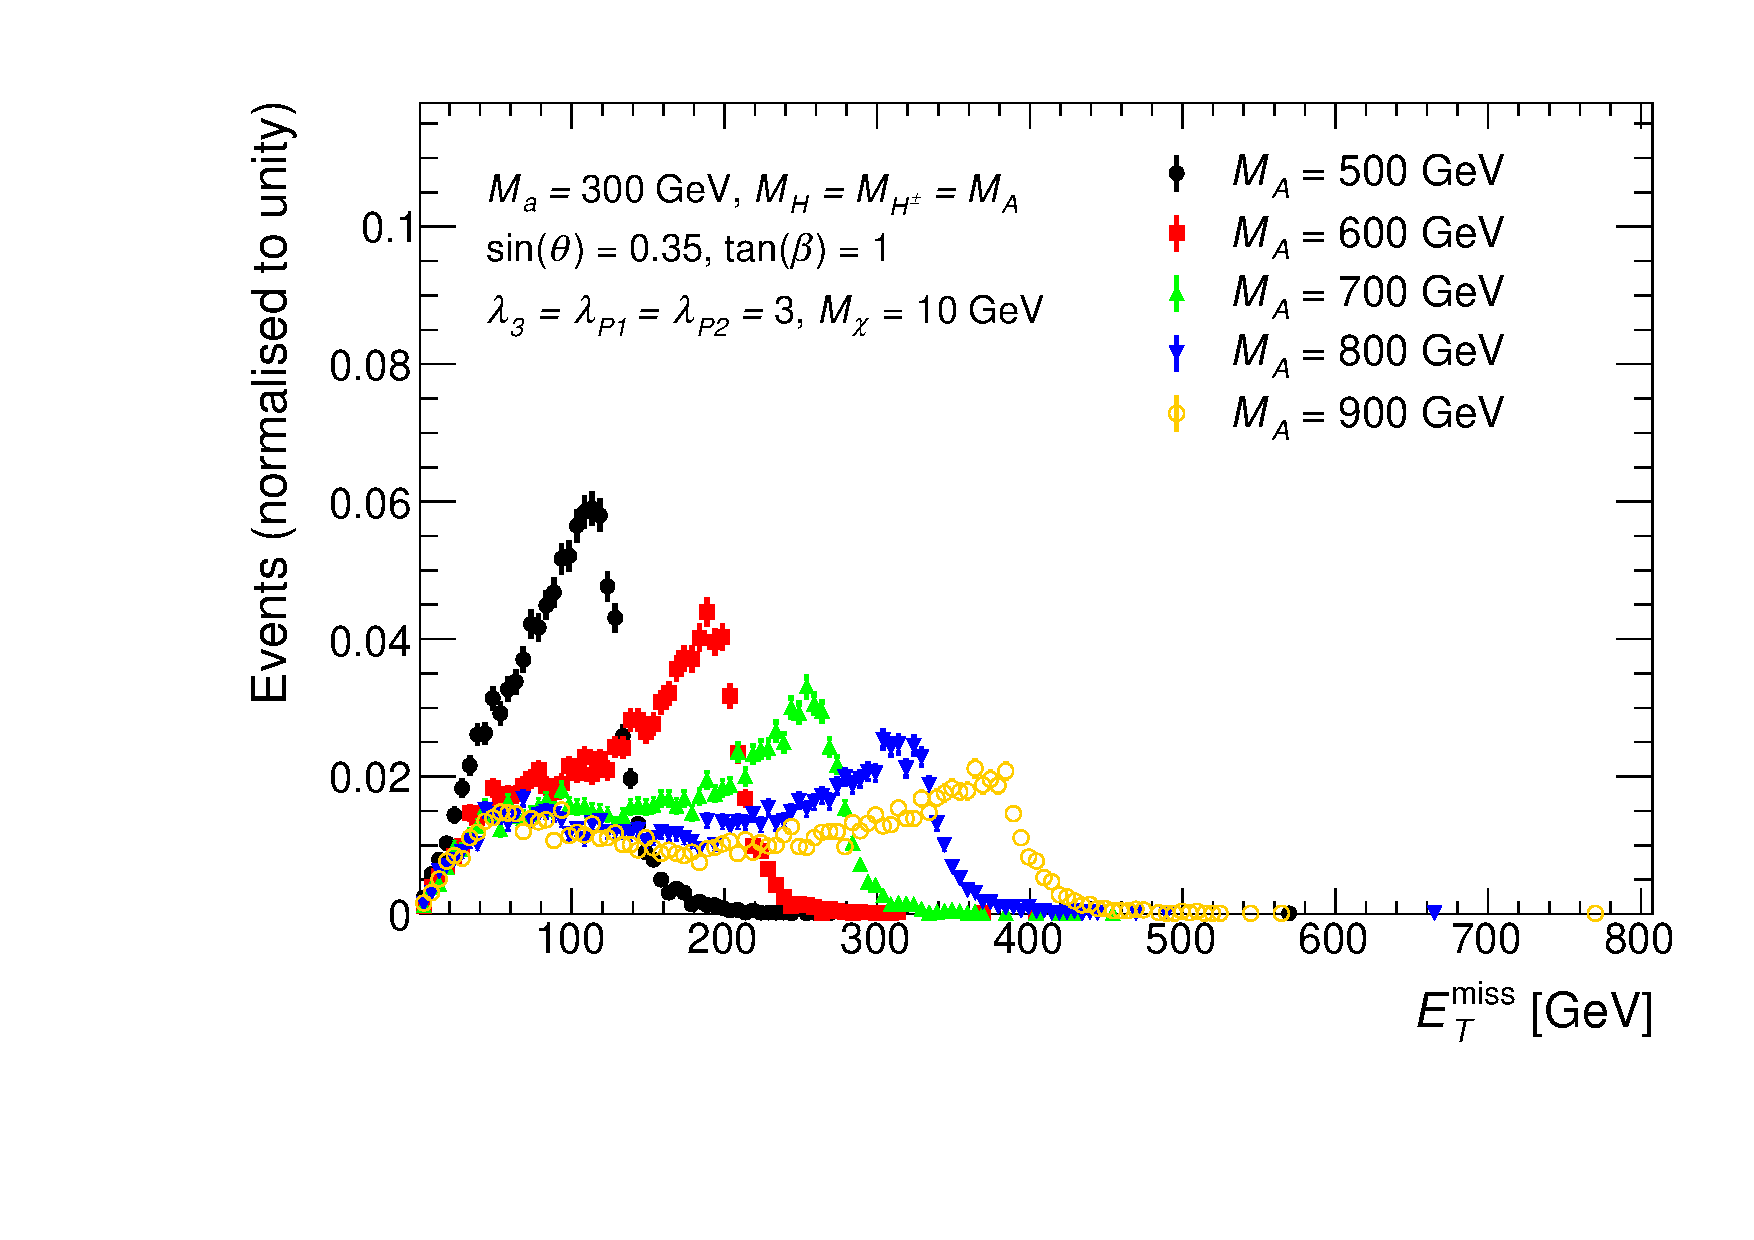
\includegraphics[width=\textwidth]{texinputs/04_grid/figures/monoHbb_m_large_A_scan_MET_liny_norm2one.pdf}
\caption[$\MET$ distribution in $h\rightarrow bb + \MET$ events for different $\mA$]
{
Missing transverse momentum distribution $h\rightarrow bb + \MET$ signal events at parton level for five representative models with different $\mA(=\mH=\mHc)$
and fixed $\ma = 300$ GeV, $ \sinp = 0.35, \tanb = 1, \mDM = 10$ GeV and $ \lap1 = \lap2 = \lam3 = 3 $. 
Models with a larger $\mA-\ma$ splitting have harder \met (s.a.  \autoref{eq:monoH_peak_met}). 
%
% interpretation for the text
%This is due to the resonant Jacobian peak shifting to higher values.}
}
\label{fig:monoHbb_mA_scan_met}
\end{figure}

\begin{figure}[tbp]
\centering
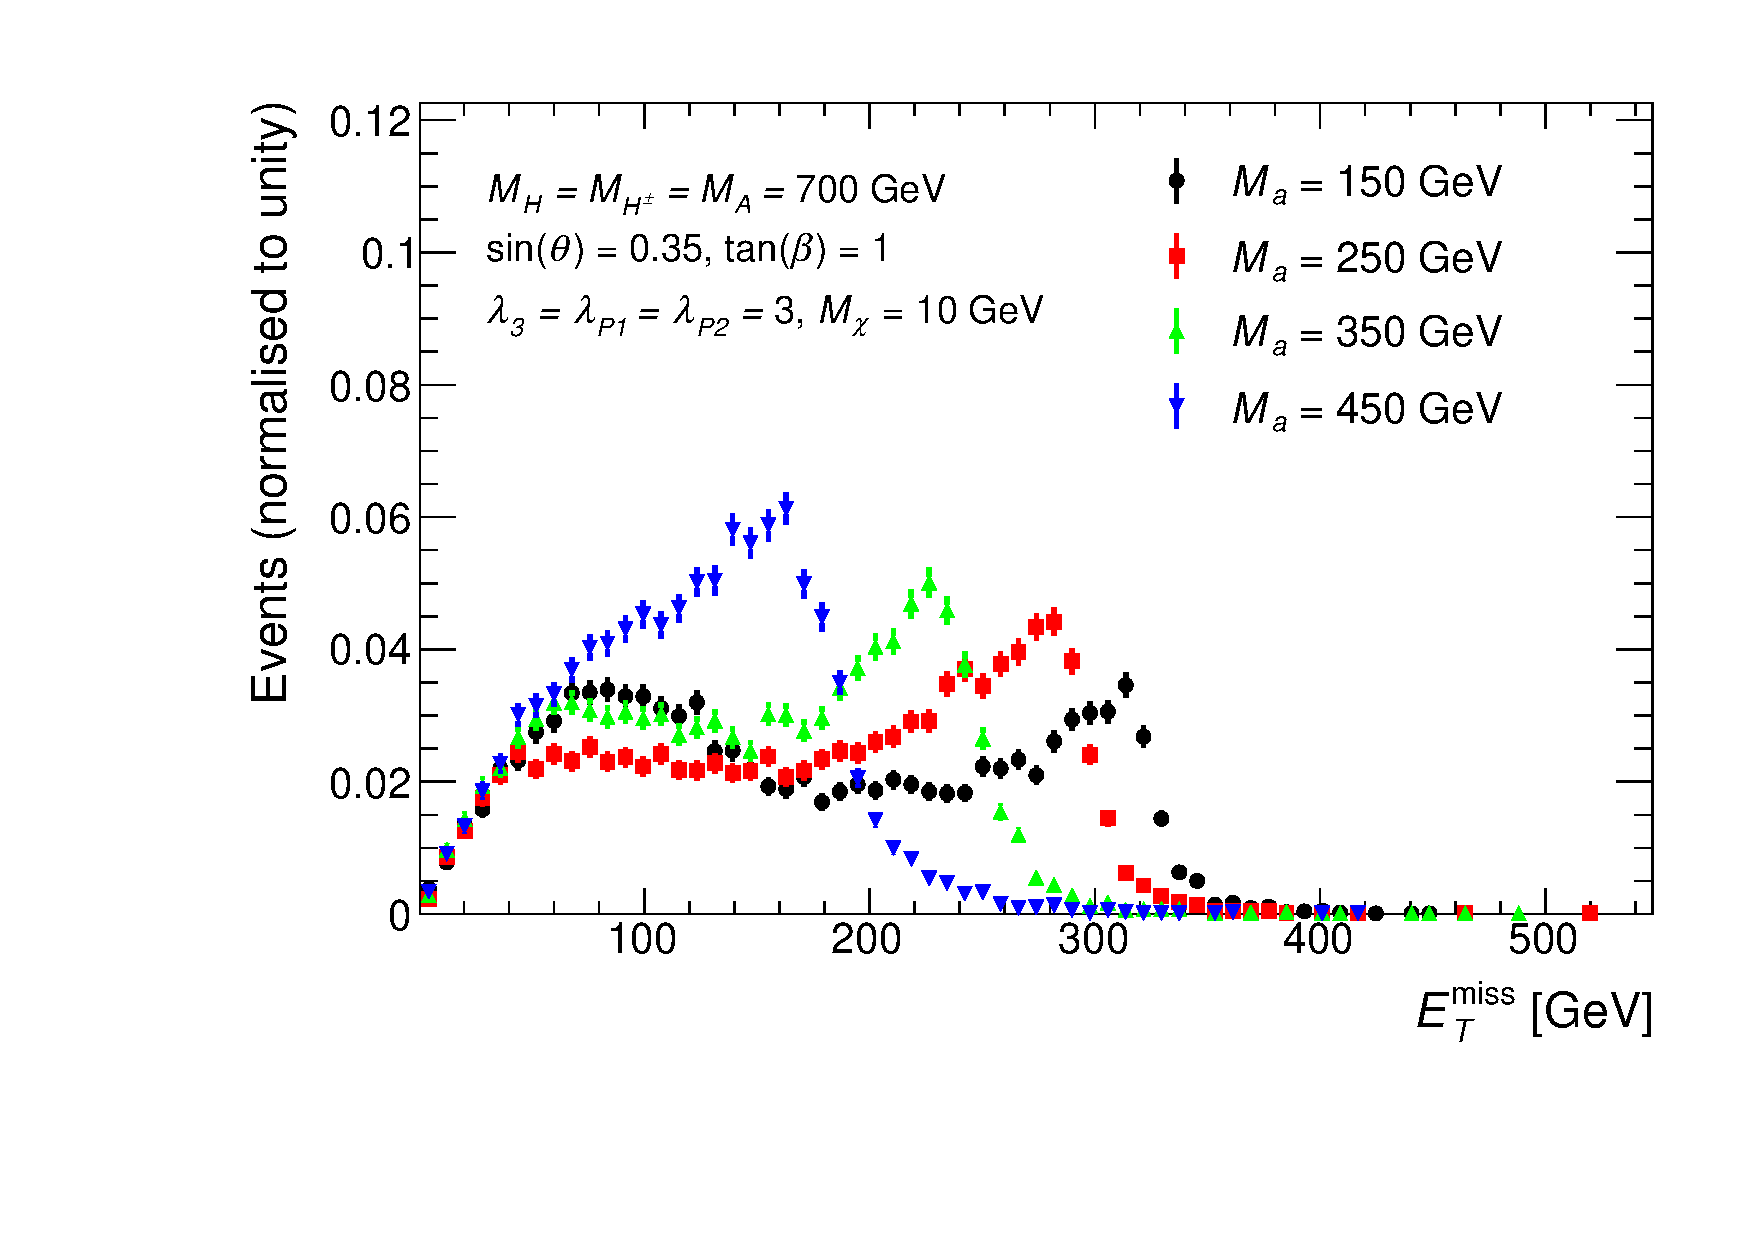
\includegraphics[width=\textwidth]{texinputs/04_grid/figures/monoHbb_m_small_a_scan_MET_liny_norm2one.pdf}
\caption[$\MET$ distribution in  $h\rightarrow bb + \MET$ events for different $\ma$]
{
Missing transverse momentum distribution in $h\rightarrow bb + \MET$ signal events at parton level for four representative models with different $\ma$ 
and fixed $ \mA=\mH=\mHc= 700$ GeV, $ \sinp = 0.35, \tanb = 1, \mDM = 10$ GeV and $ \lap1 = \lap2 = \lam3 = 3 $. 
Models with higher $\ma$ have softer \met (s.a. \autoref{eq:monoH_peak_met}).
%
% interpretation for the text
%This is due to the resonant Jacobian peak shifting to lower values.
}
\label{fig:monoHbb_ma_scan_met}
\end{figure}

\begin{figure}[tbp]
\centering
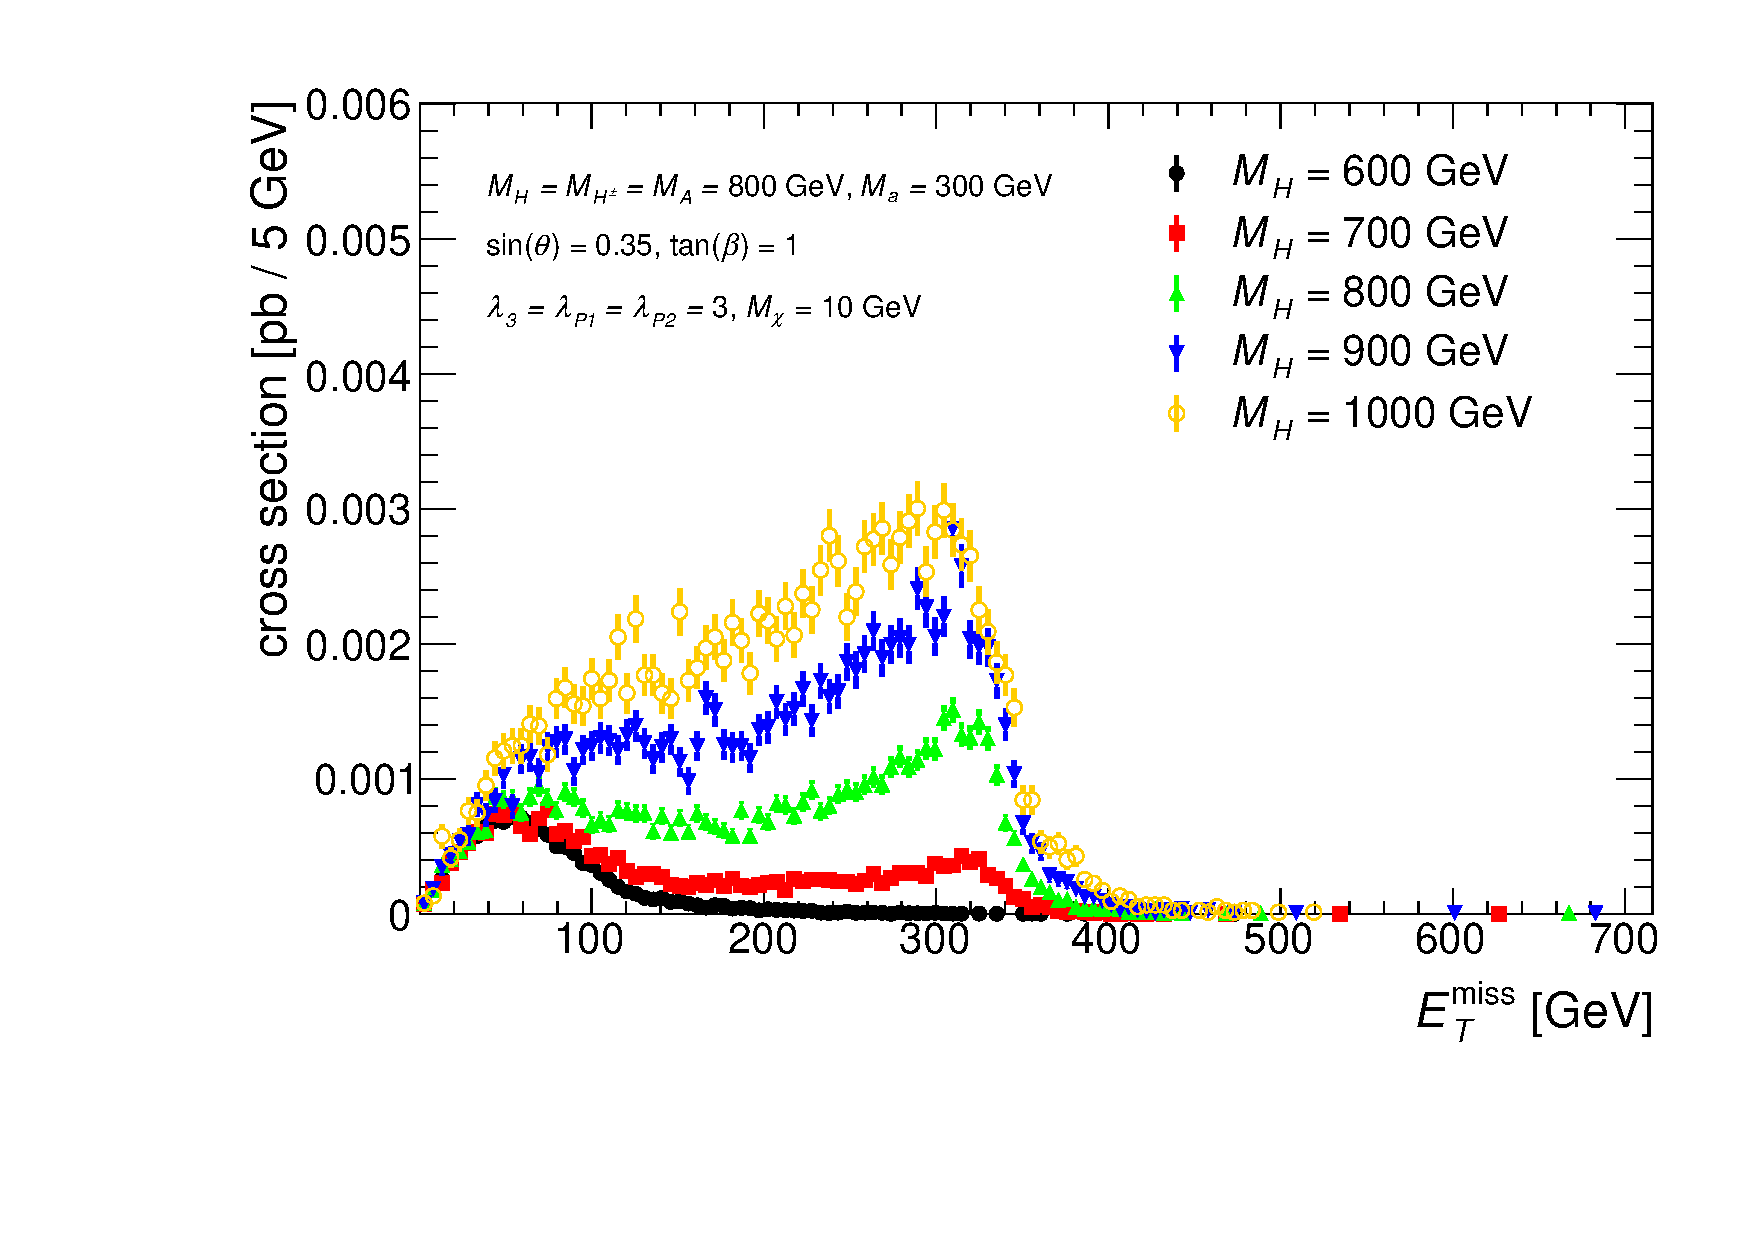
\includegraphics[width=\textwidth]{texinputs/04_grid/figures/monoHbb_mH_scan_MET_liny.pdf}
\caption[$\MET$ distribution in  $h\rightarrow bb + \MET$ events for different $\mH$]
{The \MET distribution of the production cross section of $h\rightarrow bb + \MET$ signal events for five representative models with different $\mH = \mHc$ 
and fixed $ \mA=800$ GeV, $\ma = 300 $ GeV,  $ \sinp = 0.35, \tanb = 1, \mDM = 10$ GeV and $ \lap1 = \lap2 = \lam3 = 3 $. 
%
% interpretation for the text
%Models with $\mH = \mHc \geq \mA $ have a stronger resonant contribution, and a larger cross-section. The resonant contribution is enhanced more strongly with higher $\mH = \mHc$. For $\mH = \mHc < \mA$ the resonant contribution is suppressed.
}
\label{fig:monoHbb_mH_scan_met}
\end{figure}
\begin{figure}[tbp]
\centering
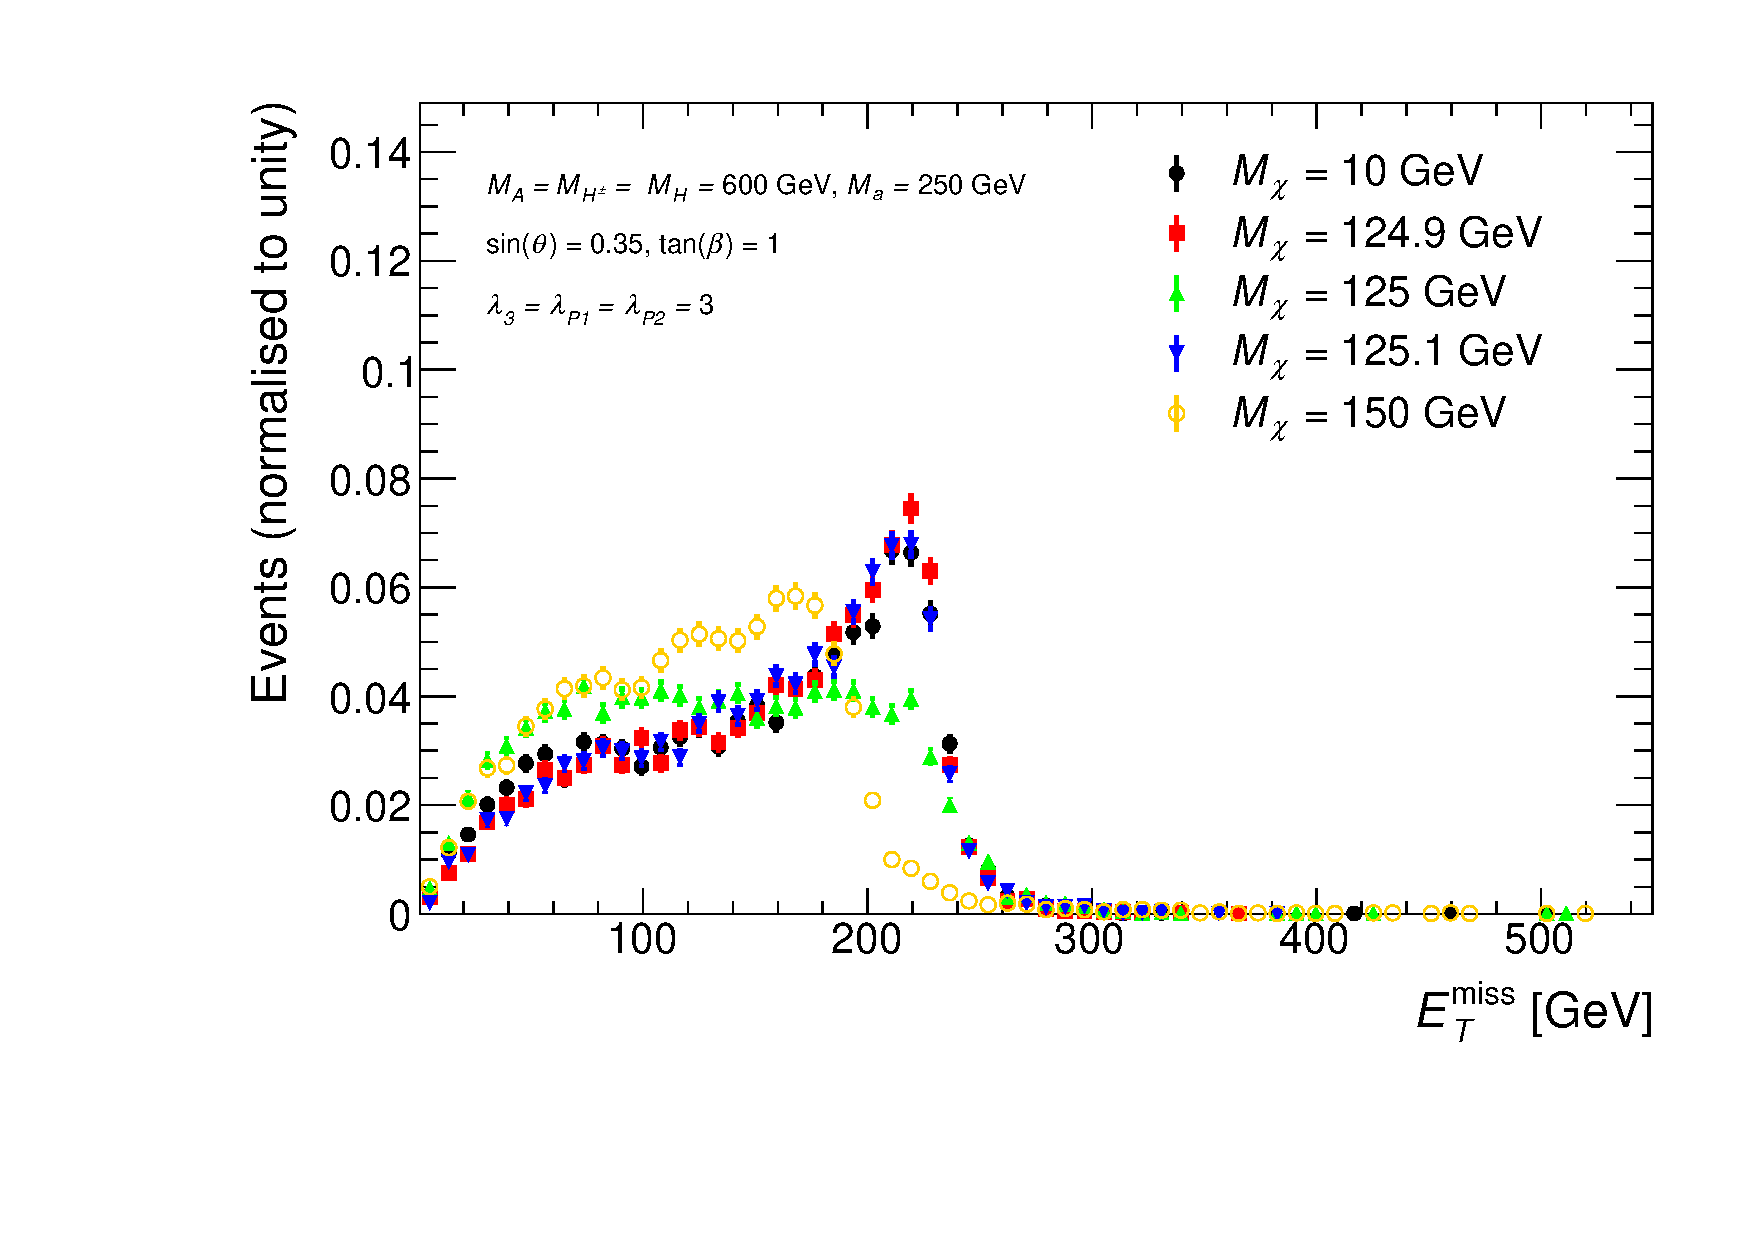
\includegraphics[width=\textwidth]{texinputs/04_grid/figures/monoHbb_mDM_scan_MET_liny_norm2one.pdf}
\caption[$\MET$ distribution in $h\rightarrow bb + \MET$ events for different $\mDM$]
{
Missing transverse momentum distribution  of $h\rightarrow bb + \MET$ signal events at parton level for five representative models with different $\mDM$
and fixed $\mA = \mH = \mHc = 600 $ GeV $\ma = 250$ GeV, $ \sinp = 0.35, \tanb = 1$ and $ \lap1 = \lap2 = \lam3 = 3 $. 
The shape of the $\MET$ distribution does not change for $\mDM < \ma/2$, then changes significantly for $\mDM>=\ma/2$.
%
}
\label{fig:monoHbb_mDM_scan_met}
\end{figure}

\begin{figure}[tbp]
\centering
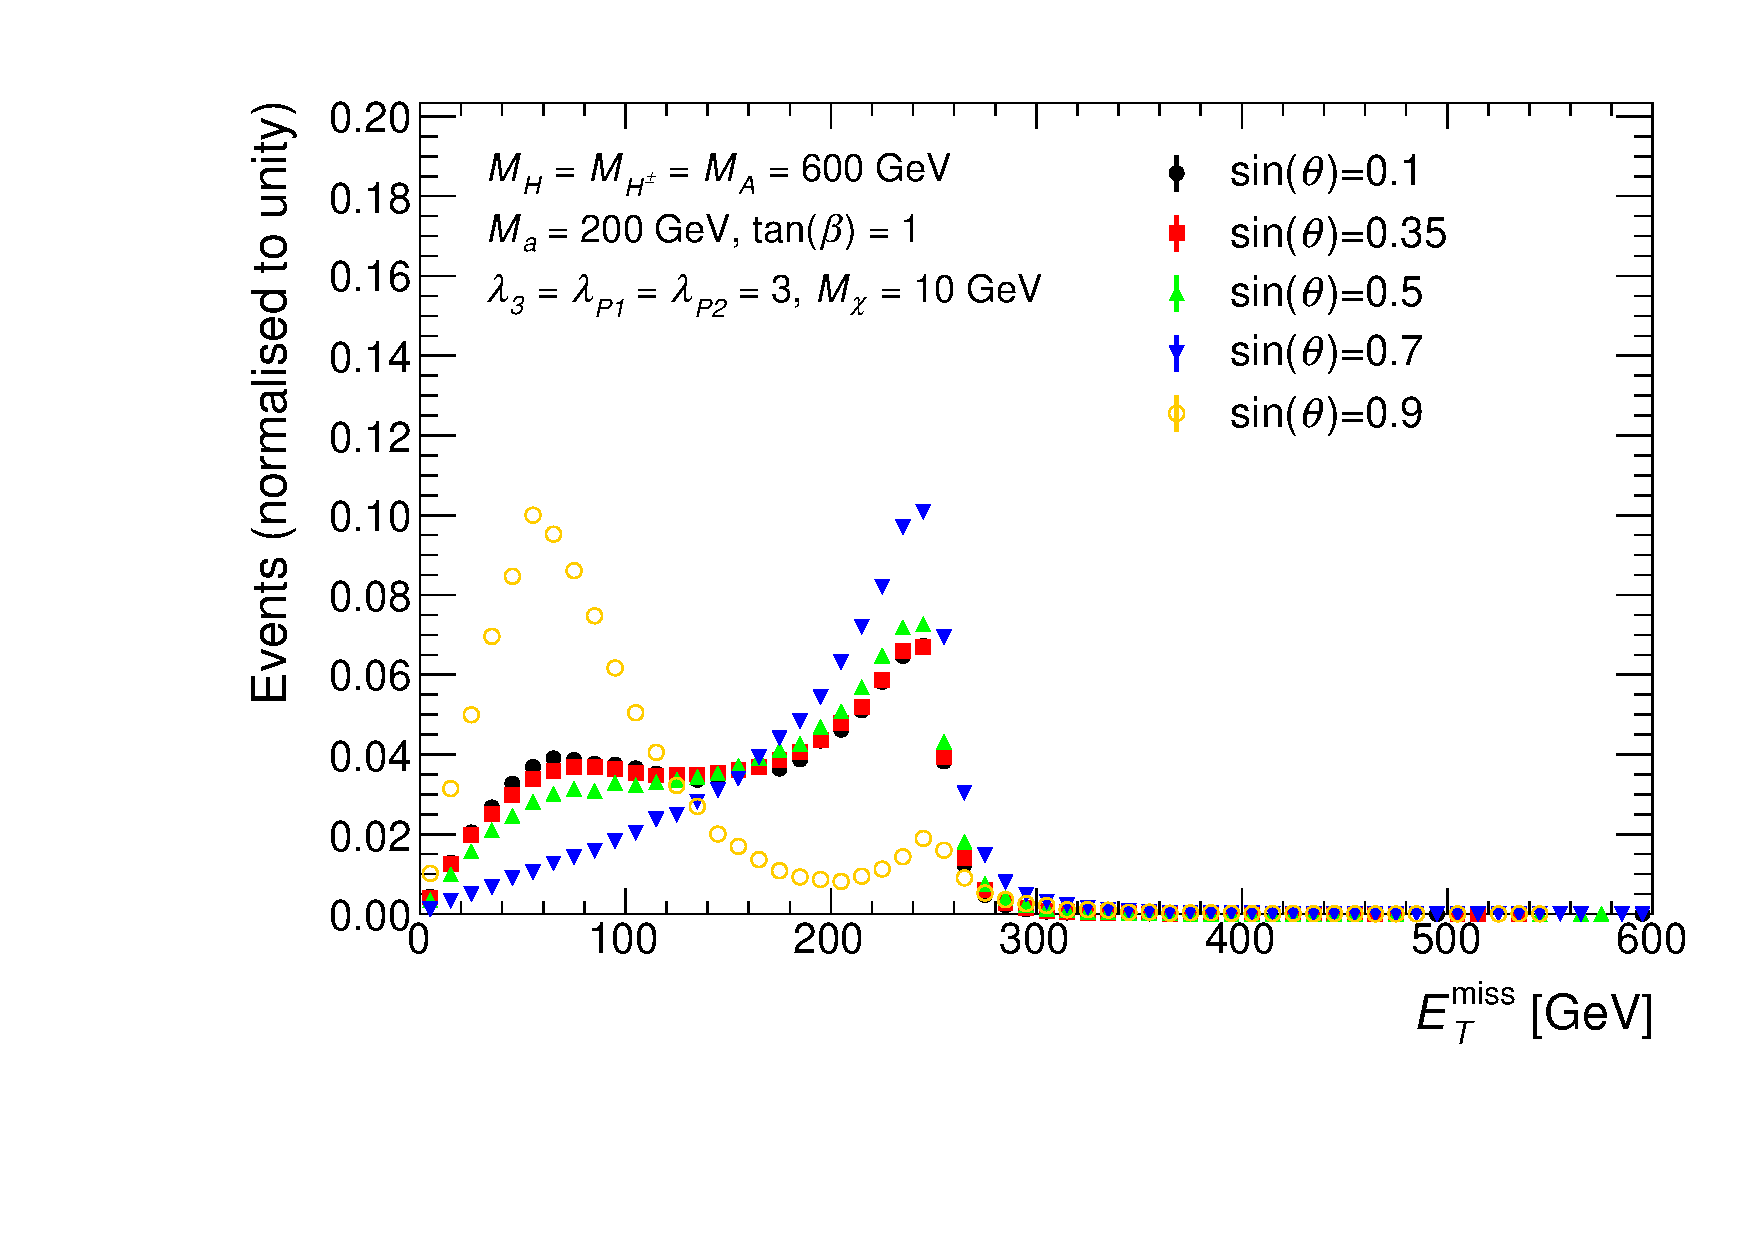
\includegraphics[width=\textwidth]{texinputs/04_grid/figures/monoHbb_sinp_scan_MA600_Ma200_MET_liny_norm2one.pdf}
\caption[$\MET$ distribution in $h\rightarrow bb + \MET$ events for different 
$\sinp$ for $\mA = \mH = \mHc = 600 $ GeV and $\ma = 200$ GeV]
{
Missing transverse momentum distribution of $h\rightarrow bb + \MET$ signal 
events at parton level for five representative models with different $\sinp$ and
 fixed $\mA = \mH = \mHc = 600 $~GeV, $\ma = 200$~GeV, $ \mDM = 10$~GeV, $\tanb = 1$, 
and $ \lap1 = \lap2 = \lam3 = 3 $. 
The shape of the $\MET$ distribution does not change much  
for $\sinp < 0.7$, then changes significantly for $\sinp\geq 0.7$. 
When $\sinp=0.9$, the diagram $gg\rightarrow a\rightarrow A^*h \rightarrow \chi \bar{\chi} h$, 
producing a \MET peak at around 60~GeV, starts to dominate.
%
}
\label{fig:monoHbb_sinp_scan_mA600_ma200_met}
\end{figure}


\begin{figure}[tbp]
\centering
\begin{subfigure}{0.48\textwidth}
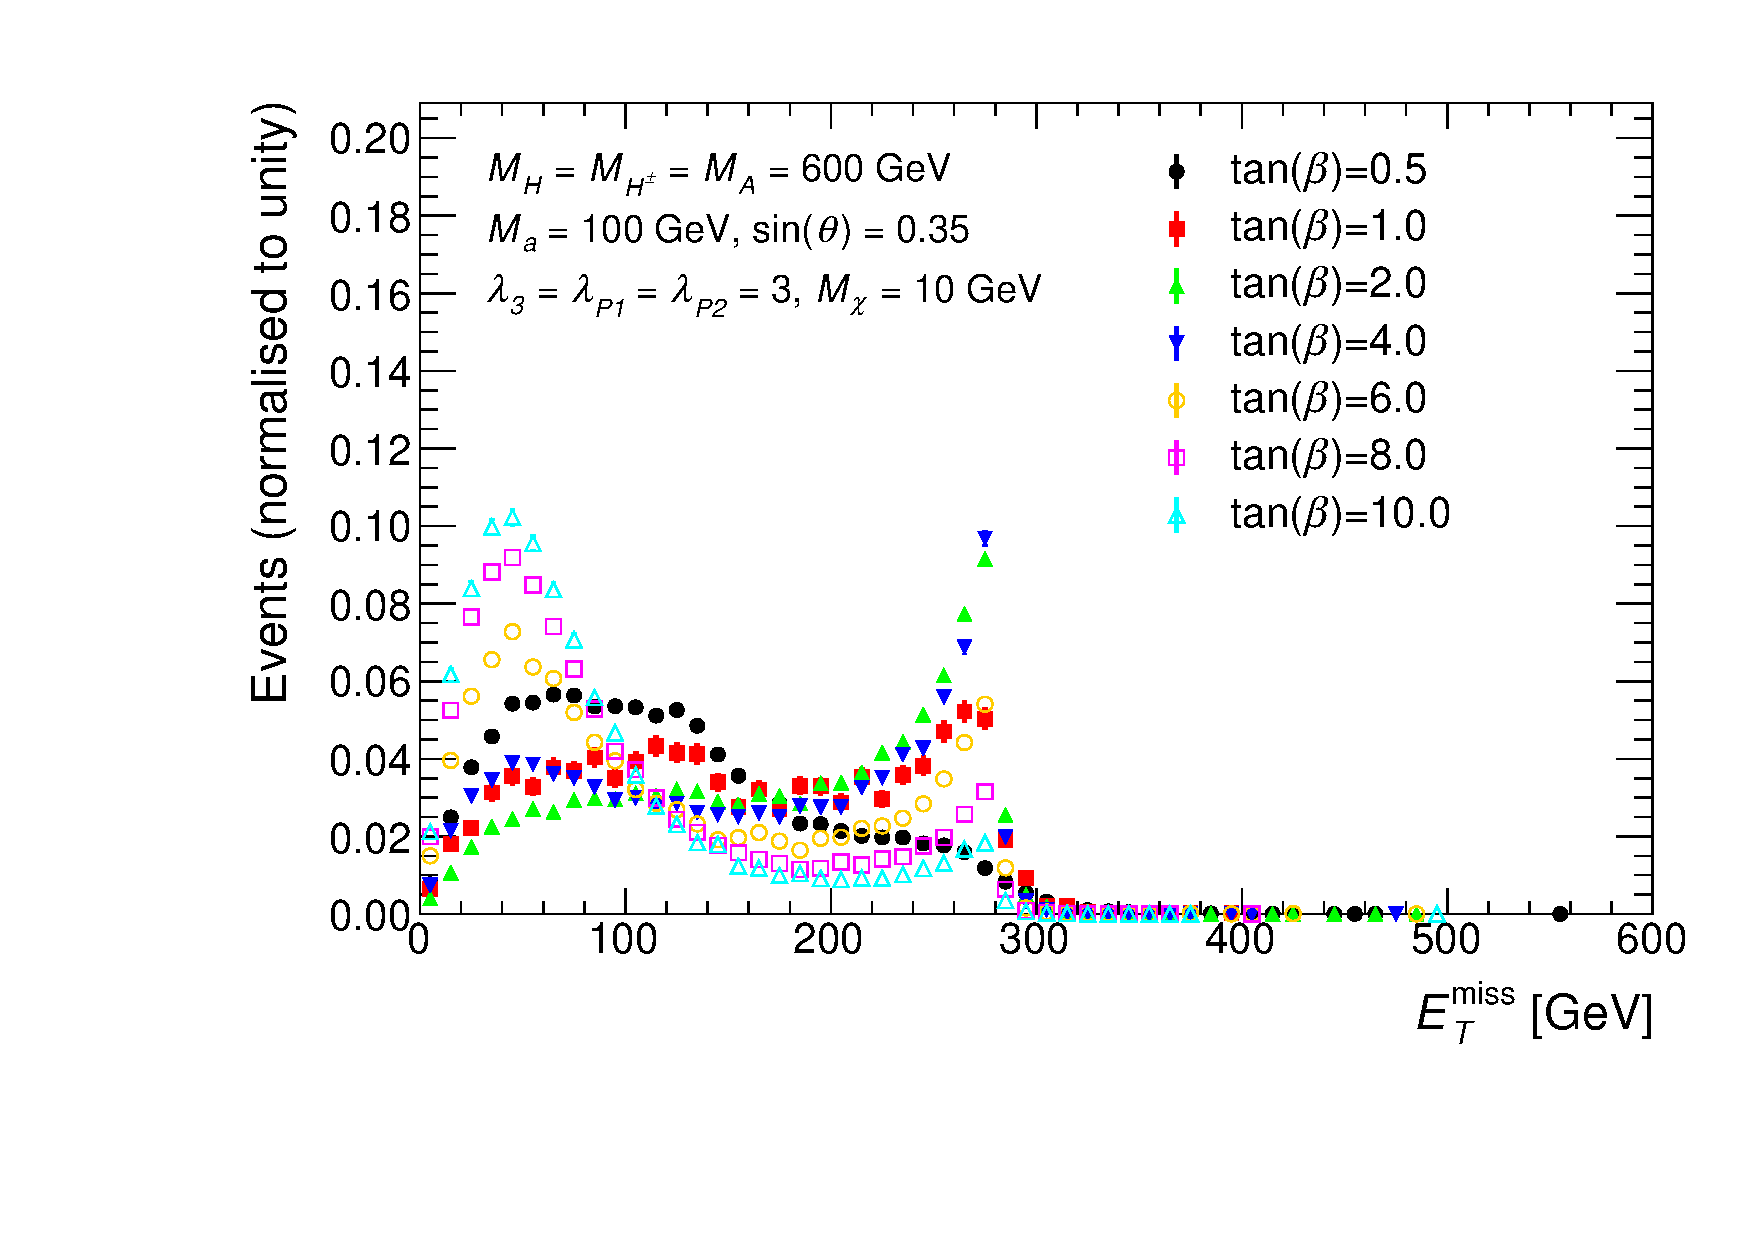
\includegraphics[width = \textwidth]{texinputs/04_grid/figures/monoHbb_tanb_scan_MA600_Ma100_MET_liny_norm2one.pdf}
\end{subfigure}
~
\begin{subfigure}{0.48\textwidth}
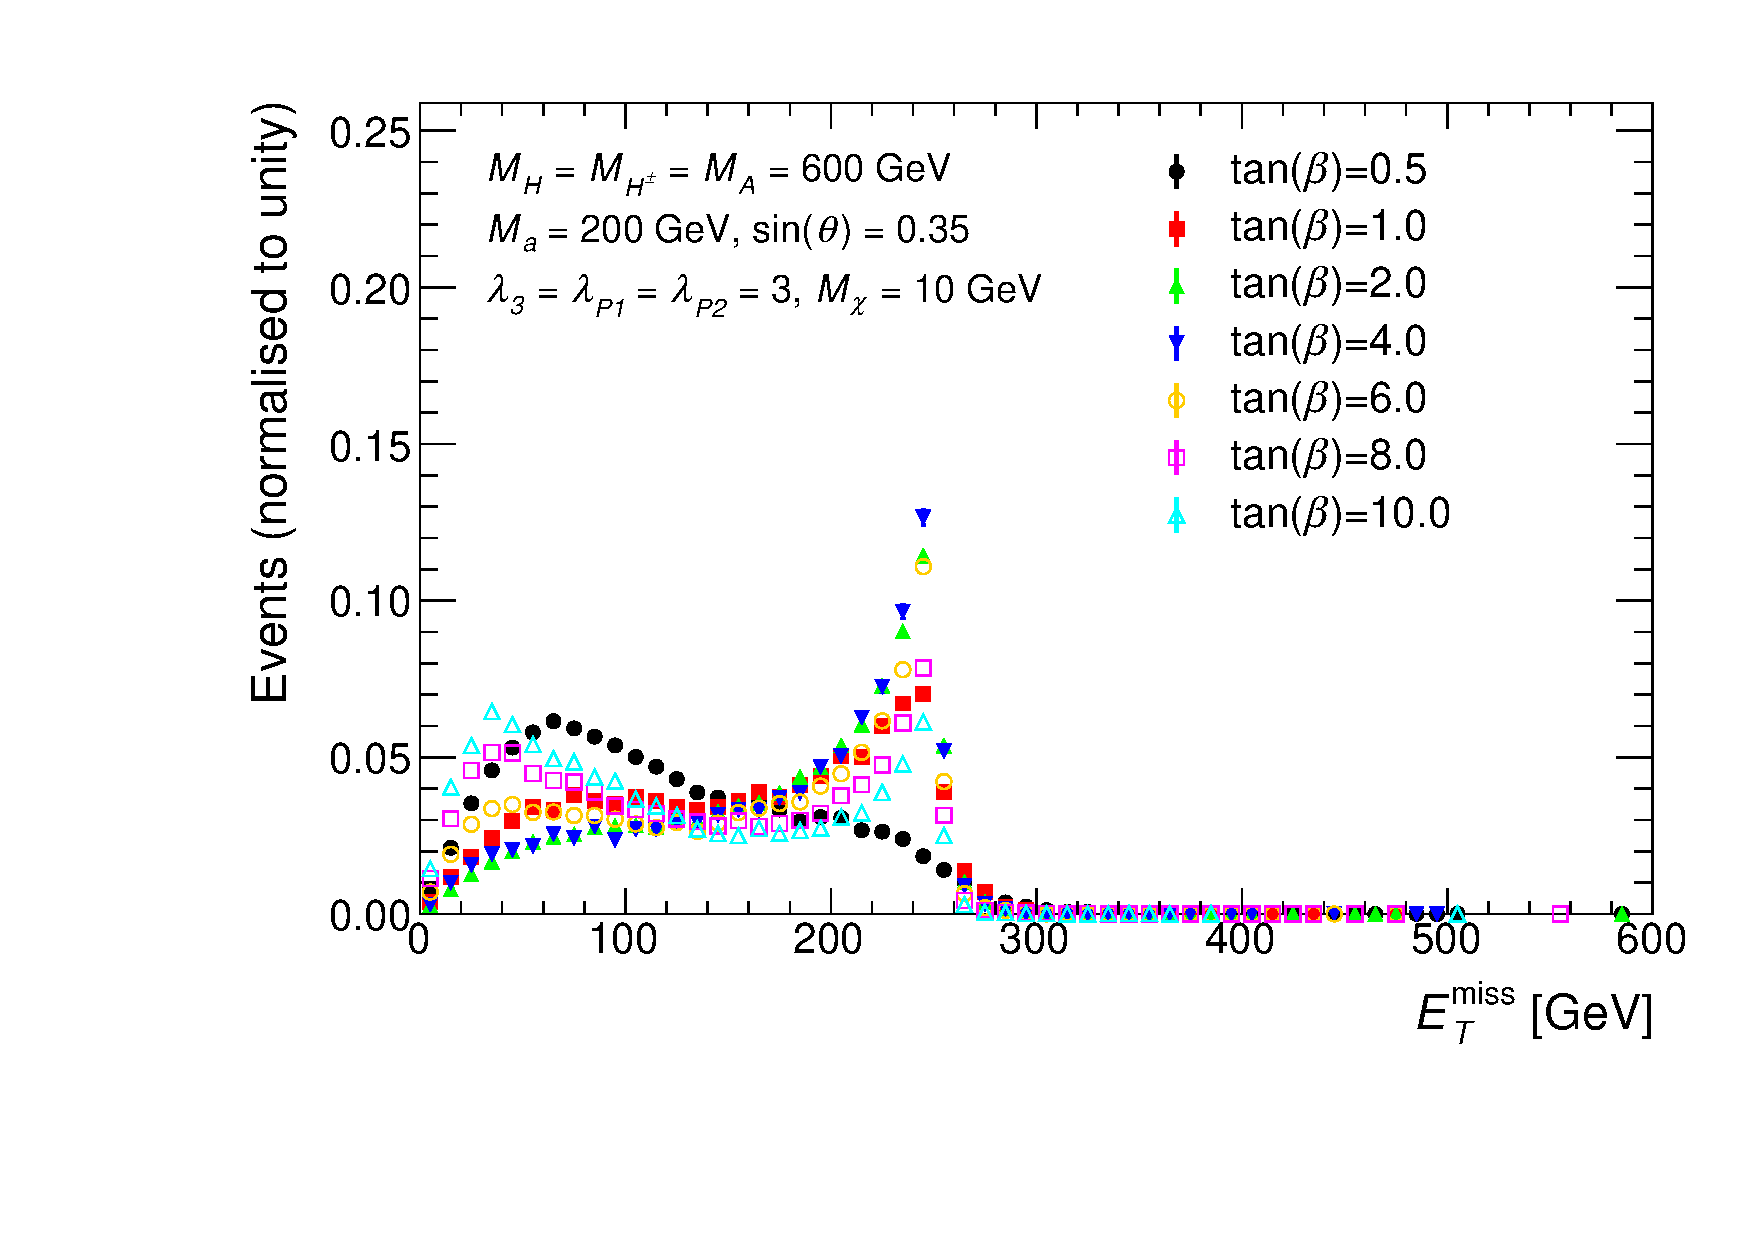
\includegraphics[width = \textwidth]{texinputs/04_grid/figures/monoHbb_tanb_scan_MA600_Ma200_MET_liny_norm2one.pdf}
\end{subfigure}
\\
\centering
\begin{subfigure}{0.48\textwidth}
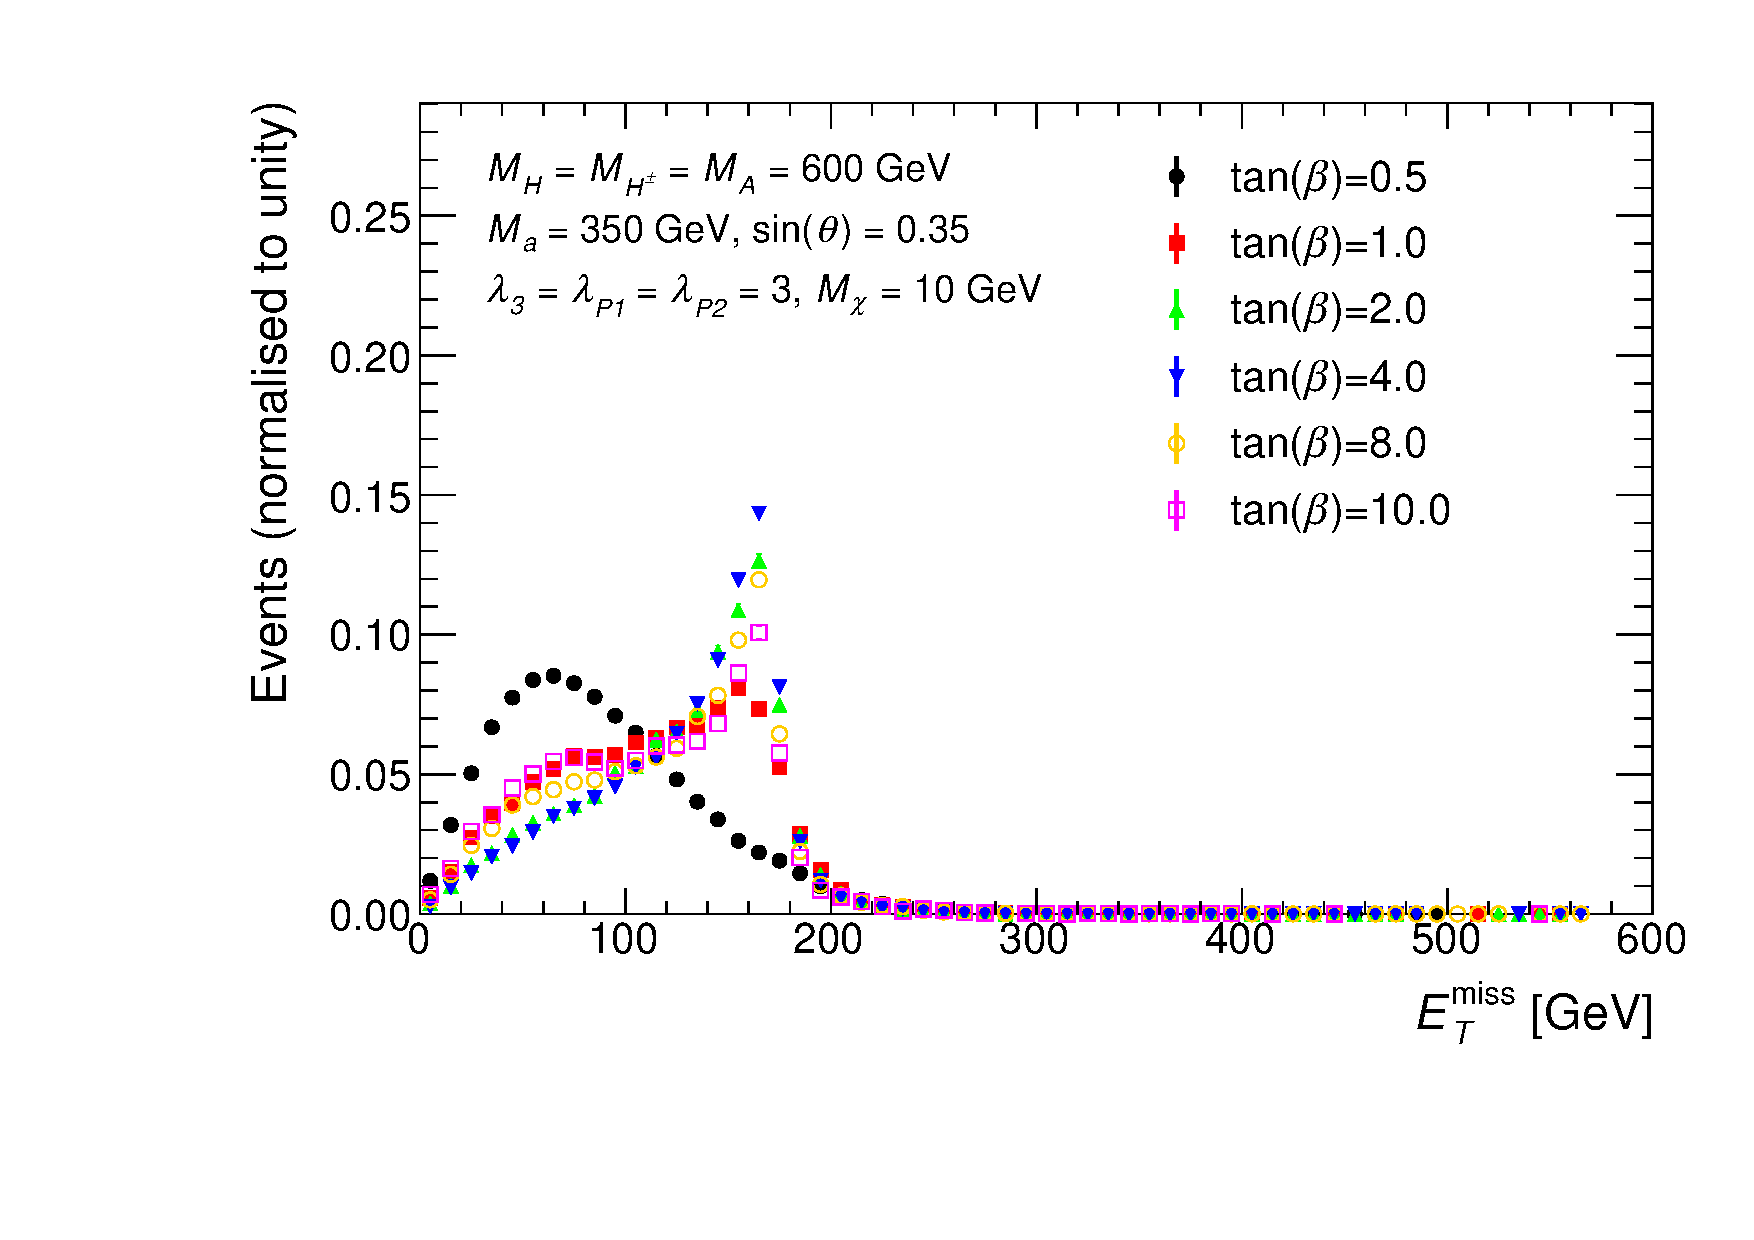
\includegraphics[width = \textwidth]{texinputs/04_grid/figures/monoHbb_tanb_scan_MA600_Ma350_MET_liny_norm2one.pdf}
\end{subfigure}
~
\begin{subfigure}{0.48\textwidth}
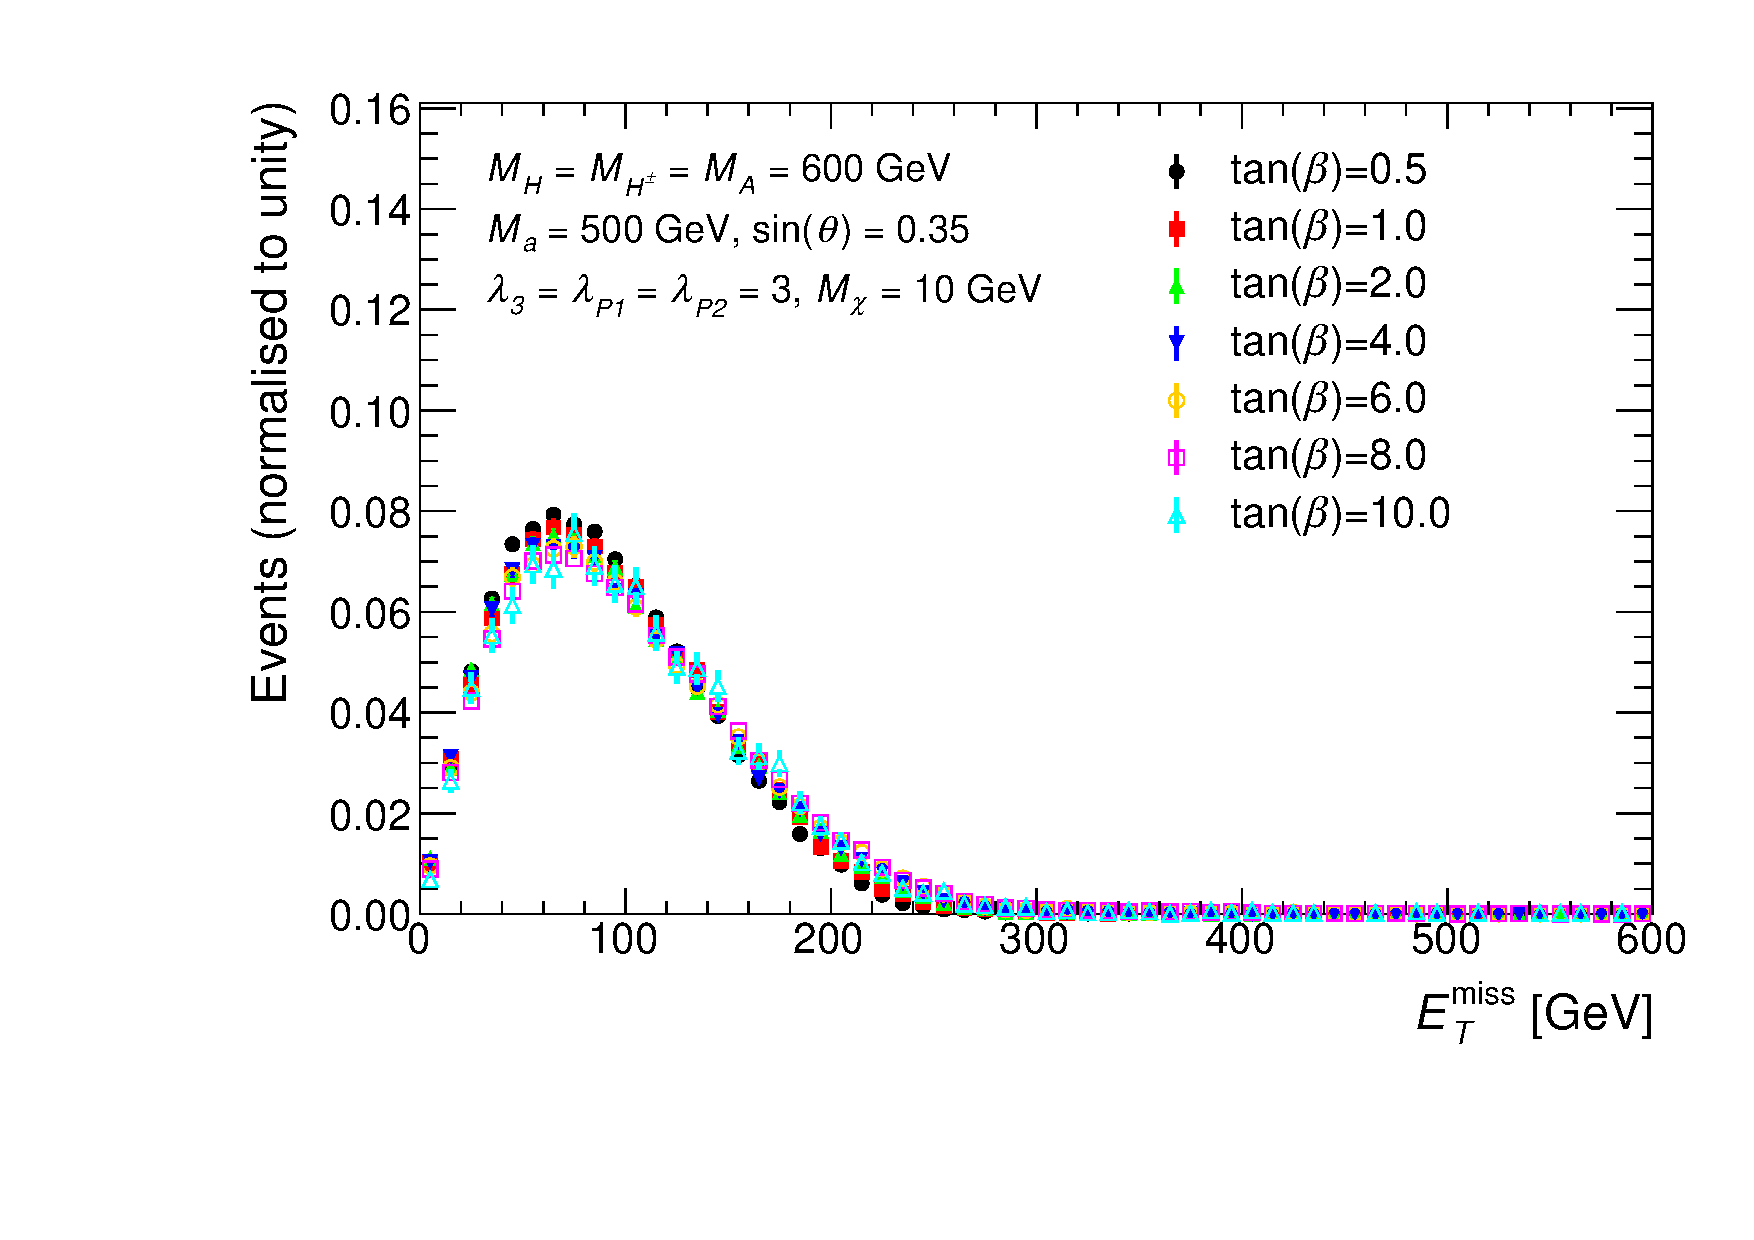
\includegraphics[width = \textwidth]{texinputs/04_grid/figures/monoHbb_tanb_scan_MA600_Ma500_MET_liny_norm2one.pdf}
\end{subfigure}
\caption[$\MET$ distribution in $h\rightarrow bb + \MET$ events for different 
$\tanb$ for $\mA = \mH = \mHc = 600 $ GeV]
{
Missing transverse momentum distribution of $h\rightarrow bb + \MET$ signal 
events at parton level with different $\tanb$ and
 fixed $\mA = \mH = \mHc = 600 $~GeV, $ \mDM = 10$~GeV, $\sinp = 0.35$, 
and $ \lap1 = \lap2 = \lam3 = 3 $. The values of $\ma$ are set to 100, 200, 
350, and 500~GeV, respectively.
The shapes of the $\MET$ distributions for different $\tanb$ are similar when 
$\mA < \mh+\ma$. Note, in these figures, both the contributions of $gg$ and $b\bar{b}$ 
initiated processes are included and a combined histogram is produced 
according to their corresponding cross sections.
}
\label{fig:monoHbb_tanb_scan_met}
\end{figure}

The masses $\mA$ and $\ma$ of the pseudoscalars $A$ and $a$ affect the $\monohbb$ signal in two ways: 
\begin{itemize}
\item by changing the location of the Jacobian peak in the \MET distribution 
\item by changing the overall signal cross-section
\end{itemize}
The latter effect can be seen in \autoref{fig:monoHbb_xsec_bins_mA_ma}. The former is crucial to searches for \monohbb such as  \cite{Aaboud:2017yqz},
since the $\MET$ observable� can be used to reduce many standard model backgrounds. 
Standard model backgrounds  are often characterized by low  $\MET$, unlike Dark Matter signal processes with potentially very high $\MET$.

The Jacobian peak is the result of a resonantly produced pseudoscalar $A$ decaying in the $1 \rightarrow 2$ decay $A\rightarrow a h$, 
where the $h$ proceeds to decay into a mostly visible final state ($h\rightarrow b \bar{b} \rightarrow \mathrm{hadrons}$), 
and the $a$ into an invisible one($a\rightarrow \chi\bar{\chi}$).
The kinematics of  $1\rightarrow 2$ processes are fixed by the masses of the involved particles.
Thus the resonant $A \rightarrow a h $  process has a sharply peaked resonance\footnote{with a finite width due to the widths of a, A and h} 
in the invariant mass distribution of the final state system. This results in a  peak in the momentum distribution of the Dark Matter system,
and the transverse component of the Dark Matter momentum is reconstructed as the missing transverse momentum ($\MET$).
This peak in the $\MET$ distribution resulting from the resonant signal process  is called the Jacobian peak.

Since it is determined by the masses of the particle involved in the signal process, 
the location of the Jacobian peak can be calculated analytically \cite{Bauer:2017ota}:
\begin{align}
E^{\mathrm{miss},max}_T \approx \frac{\sqrt{\left(\mA^2 -\ma^2 -M_{h}^2\right)^2 - 4 \ma^2 M_{h}^2}}{2\mA}  \label{eq:monoH_peak_met}
\end{align}
Thus increasing $\mA$ leads to a Jacobian peak at higher $\MET$, and vice versa (\autoref{fig:monoHbb_mA_scan_met}).
Conversely, models with higher $\ma$ have a Jacobian peak at lower $\MET$, and vice versa (\autoref{fig:monoHbb_ma_scan_met}). 
Because they determine the location of the Jacobian peak, $\mA$ and $\ma$ strongly affect the sensitivity of a search for \monohbb to a given model.
For this reason, one of the proposed parameter scans for the 2HDM with pseudoscalar Dark Matter  mediator is a scan in the ($\ma$,$\mA$) plane.

Some fraction of signal events is due to non-resonant $2 \rightarrow 3$ processes $gg \rightarrow h \chi \bar{\chi}$. 
%link into thereory section graph or cite paper
Due to the larger number of kinematic degrees of freedom, these processes have a broadly distributed  invariant mass of the final state system.
This in turn generates a broad distribution dominated by soft $\MET$, distinct from the Jacobian peak discussed above.
All the models in \autoref{fig:monoHbb_mA_scan_met} and \autoref{fig:monoHbb_ma_scan_met} also have low-$\MET$ non-resonant contributions.

The mass of the heavy neutral\footnote{For simplicity, we only consider the case of the neutral scalar $H^{\pm}$ being mass-degenerate to $H$.} 
scalar $H$ has an indirect effect on the rate and kinematics of the signal. 
This is caused by  $\mH$ changing the widths and couplings of  the pseudoscalars $A$ and $a$. 
Changing $\mH$ can scale the signal cross-section up or down, and change the 
fraction of resonant vs. non-resonant signal events (\autoref{fig:monoHbb_mH_scan_met}). 
The choice $\mH (= \mHc) = \mA$ gives a measurable cross-section for many signal points as well as a significant fraction of resonant signal events.

The mass  $\mH$ of the Dark Matter fermion $\mDM$ can change the cross-section and shape of the $\MET$ distribution,
depending on the place of $\mDM$ in the mass hierarchy (\autoref{fig:monoHbb_mDM_scan_met}). 
If the Dark Matter is above the production threshold ($\mDM < \ma/2$), changing it has no effect on either kinematics or cross-section. 
The only exception is the case $\ma/2 > \mDM > \ma/2 - M_h$ (given a sufficiently heavy scalar $a$). With such values of $\mDM$
non-resonantly producing an $h$ simultaneously with an on-shell $a (\rightarrow \chi \bar{\chi})$ becomes kinematically forbidden. 
However, this contribution is negligible for most of the parameter points in the scans presented here. 
If the Dark Matter is on threshold ($\mDM = \ma/2$), the signal cross section is significantly enhanced. 
This enhancement on threshold drops off rapidly towards both higher and lower $\mDM$. Furthermore, the shape of the $\MET$ distribution at threshold 
differs significantly from the one below threshold, since amplitudes involving decays $a\rightarrow\chi\bar{\chi}$ 
make up a larger fraction of all signal events. Below threshold ($\mDM > \ma/2$), 
the signal cross-section quickly drops by several orders of magnitude. In this regime, 
the shape of the $\MET$ distribution changes with $\mDM$ continuously.

%%%%% text related to scan of sinp
The sine of the mixing angle between the two pseudoscalars $A$ and $a$, $\sinp$,
affects not only the cross section, but also the shape of the \MET\ distribution 
(\autoref{fig:monoHbb_sinp_scan_mA600_ma200_met}). 
For the resonant diagram $gg\rightarrow A \rightarrow ah \rightarrow \chi\bar{\chi}h$, 
the product of cross section times branching ratios 
${\cal B}(A\rightarrow ah){\cal B}(a \rightarrow \chi\bar{\chi})$ 
scales with $\sin^2\theta\cos^6\theta$, while for the diagram 
$gg\rightarrow a \rightarrow A^*h \rightarrow \chi\bar{\chi}h$, the 
product of cross section times branching ratios 
${\cal B}(a\rightarrow Ah){\cal B}(A \rightarrow \chi\bar{\chi})$ 
scales with $\sin^6\theta\cos^2\theta$. Therefore, at small \sinp, the resonant 
diagram $A\rightarrow ah$ is the dominant production mode and the \MET\ distribution 
has a Jacobian peak following \autoref{eq:monoH_peak_met}; while at large \sinp, the 
$a\rightarrow A^*h$ diagram starts to dominate and produces a second peak at a lower 
\MET\ value.

%%% text related to tanbeta-ma scan
The shape of \MET\ distribution also has a non-trivial dependence on \tanb\ 
(\autoref{fig:monoHbb_tanb_scan_met}).
As discussed in the sensitivity study later, at small \tanb, the Yukawa coupling 
to top quark is large and the signal production mode is dominated by the 
non-resonant 3-body processes $gg\rightarrow h\chi\bar{\chi}$, which gives a broad 
and soft \MET\ spectrum. As \tanb increases, the contribution of 
resonant production increases as well and the Jacobian peak also appears.
When the pseudoscalar $A$ is produced off-shell, i.e. when $\mA<\ma+\mh$, the shapes 
of \MET\ distributions become similar and the dependence on \tanb disappears.


\subparagraph{Sensitivity estimate}
\begin{figure}[tbp]
\centering
\begin{subfigure}{0.48\textwidth}
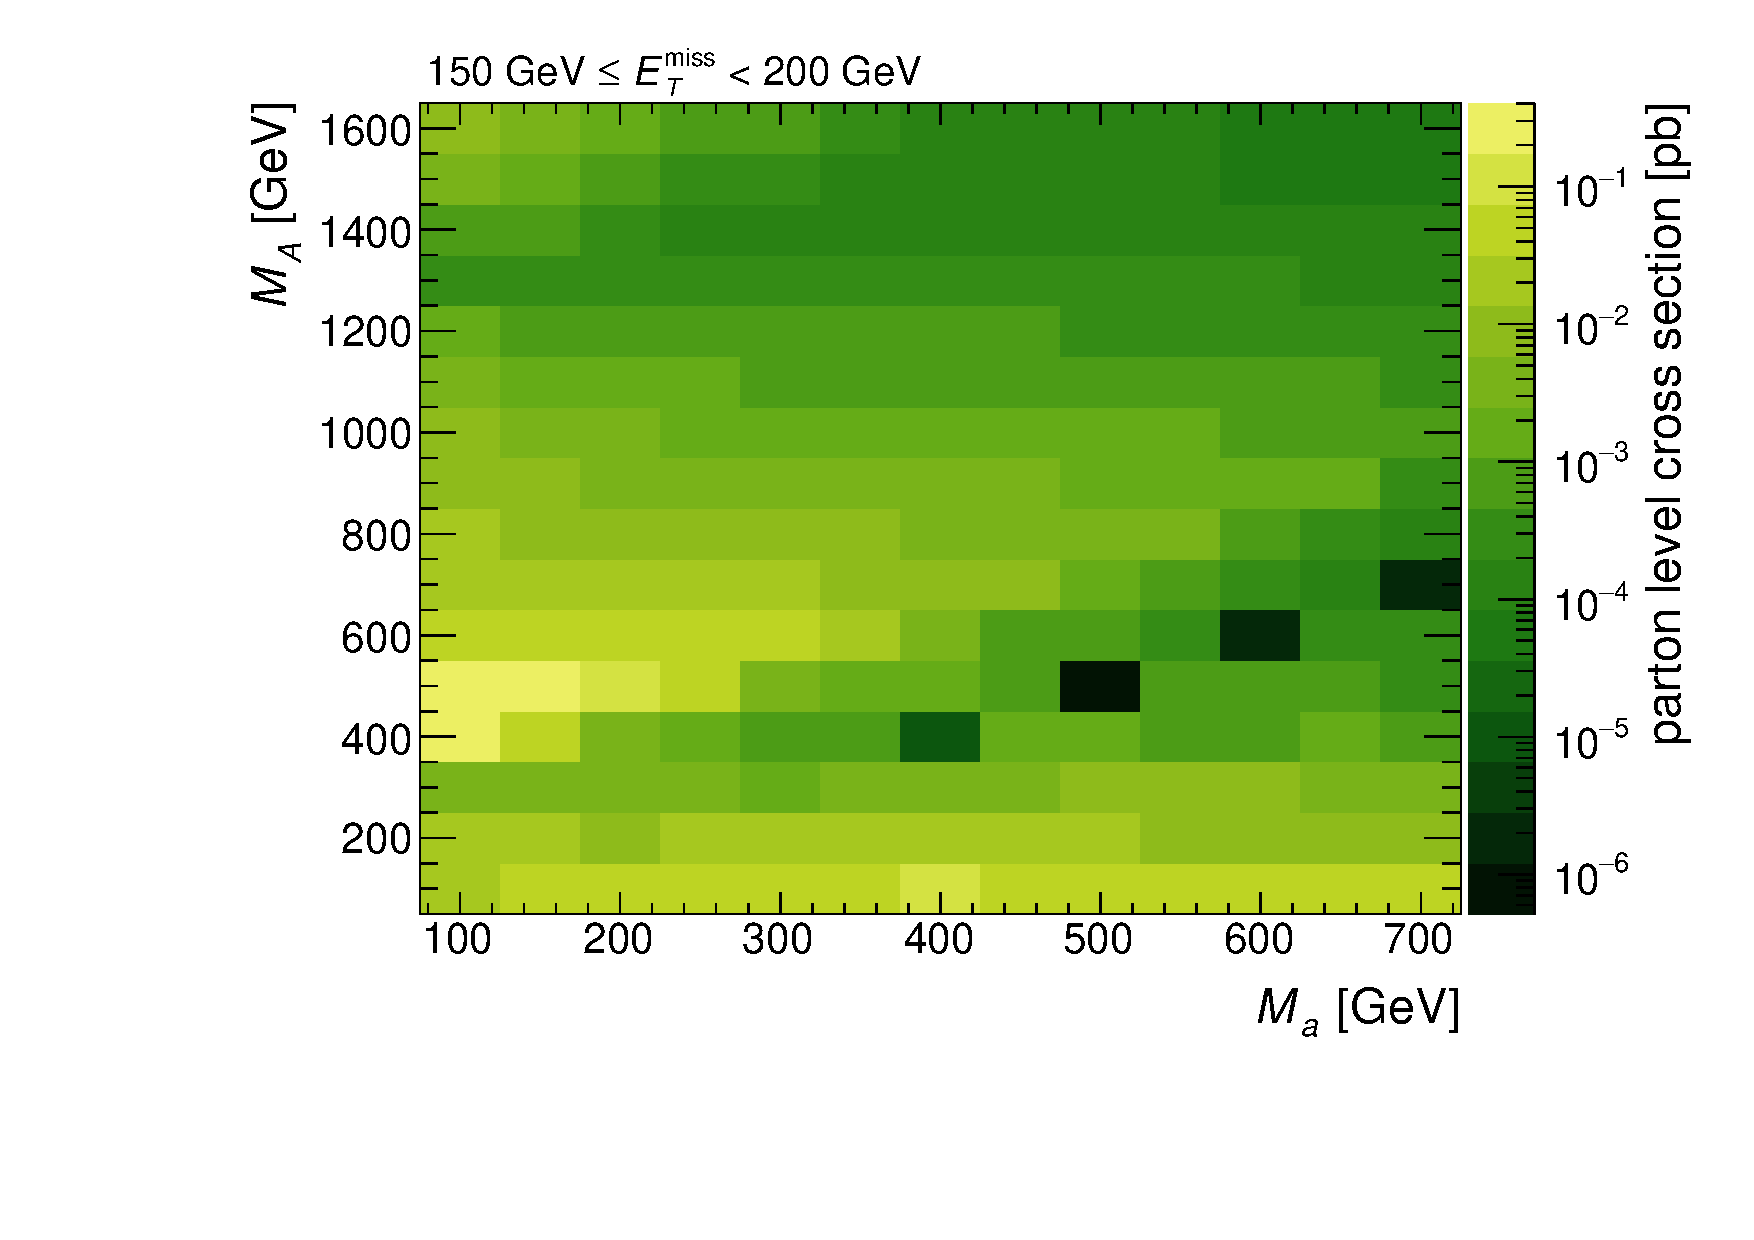
\includegraphics[width = \textwidth]{texinputs/04_grid/figures/monoHbb_parton_level_cross_section_bin_1_ma_vs_mA_lin.pdf}
\end{subfigure}
~
\begin{subfigure}{0.48\textwidth}
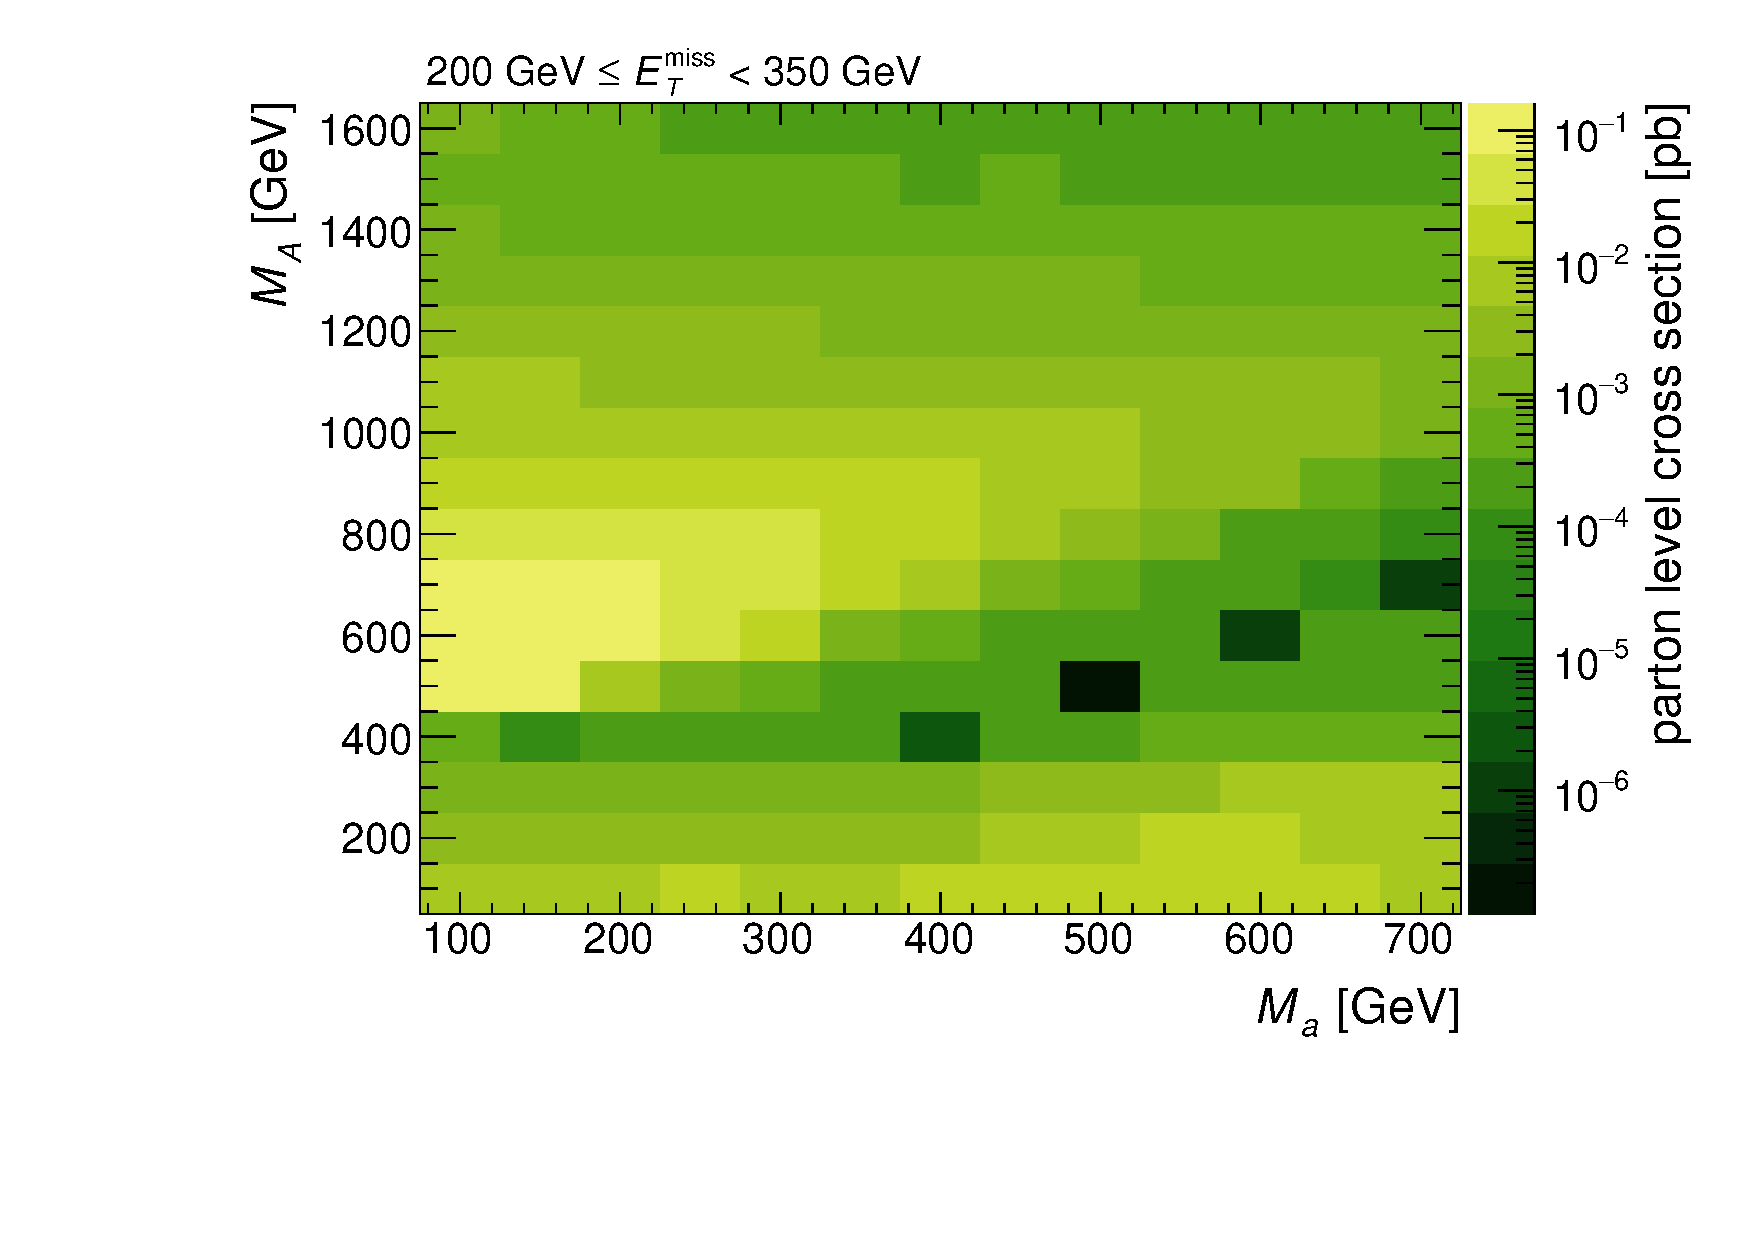
\includegraphics[width = \textwidth]{texinputs/04_grid/figures/monoHbb_parton_level_cross_section_bin_2_ma_vs_mA_lin.pdf}
\end{subfigure}
\\
\centering
\begin{subfigure}{0.48\textwidth}
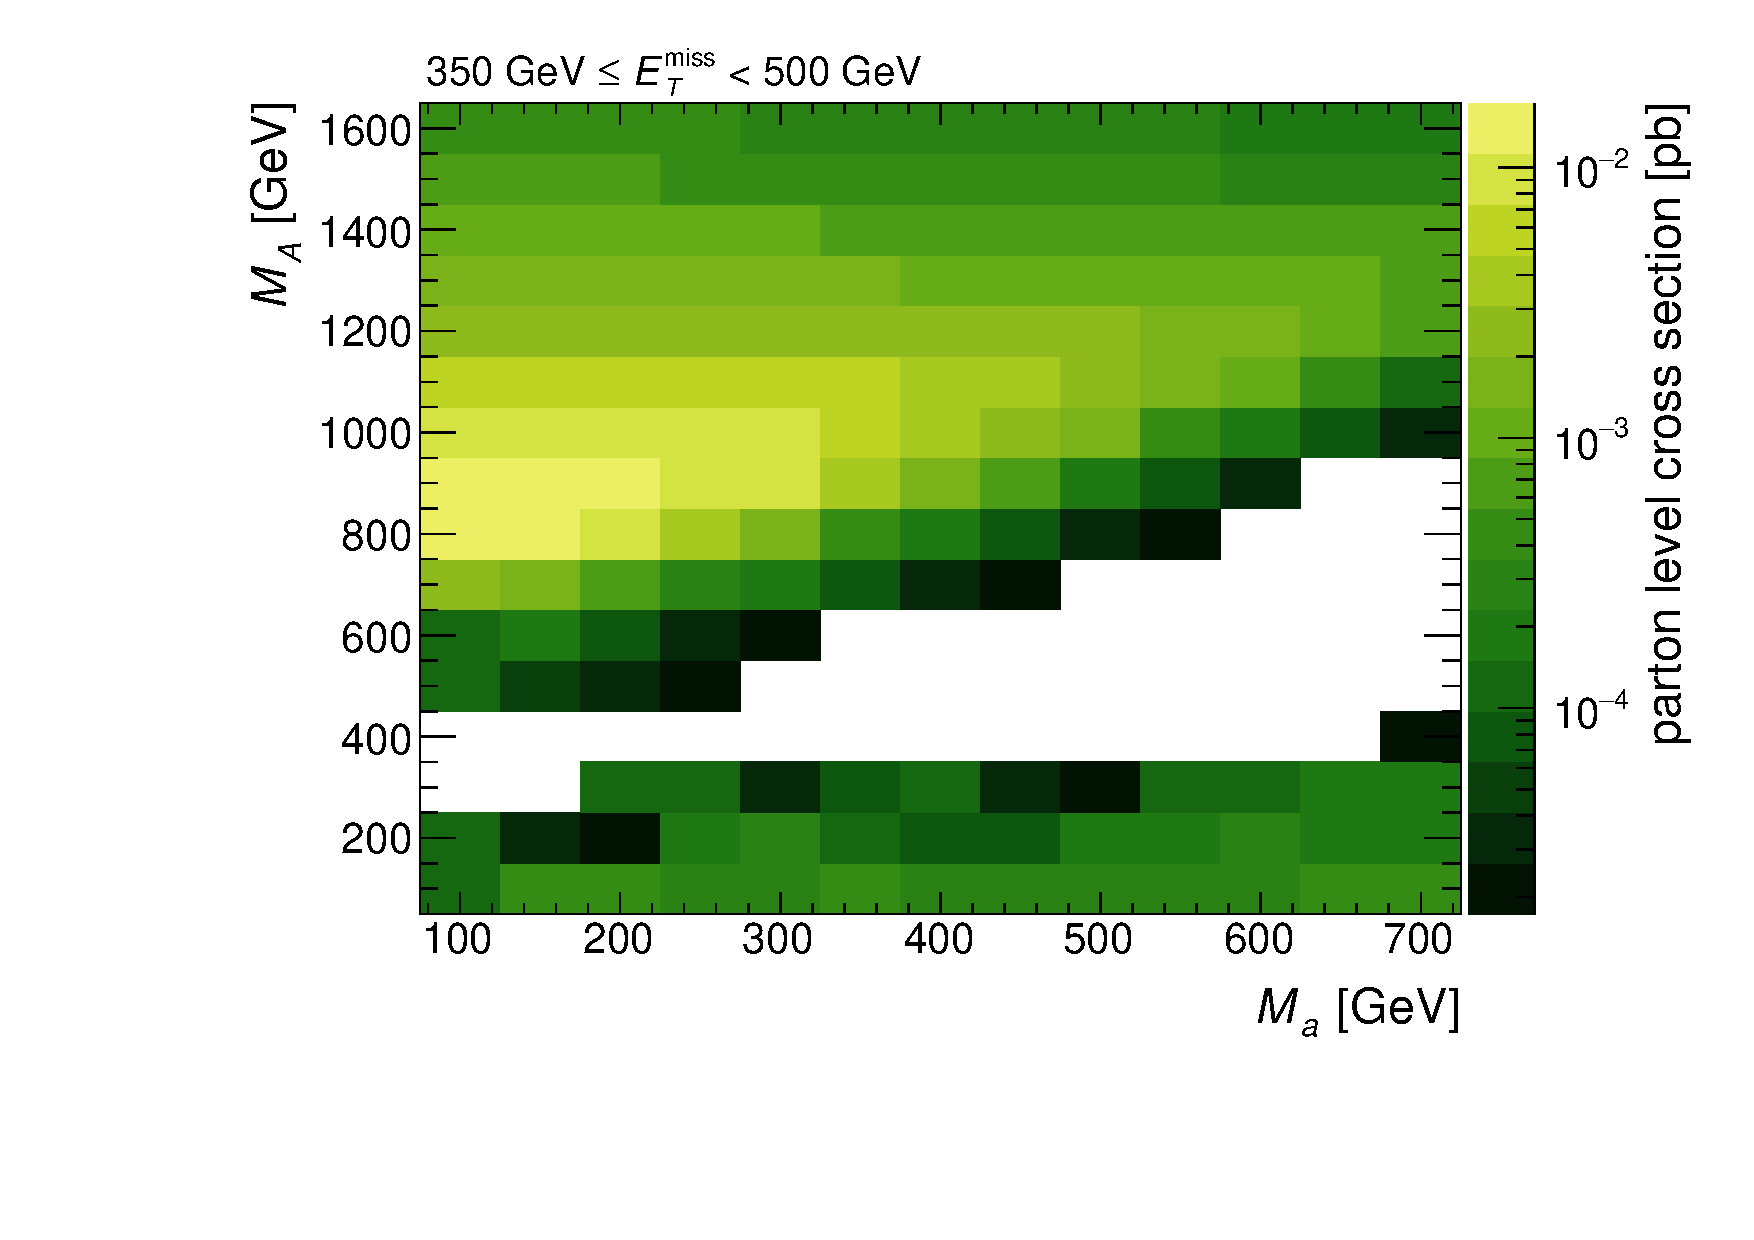
\includegraphics[width = \textwidth]{texinputs/04_grid/figures/monoHbb_parton_level_cross_section_bin_3_ma_vs_mA_lin.pdf}
\end{subfigure}
~
\begin{subfigure}{0.48\textwidth}
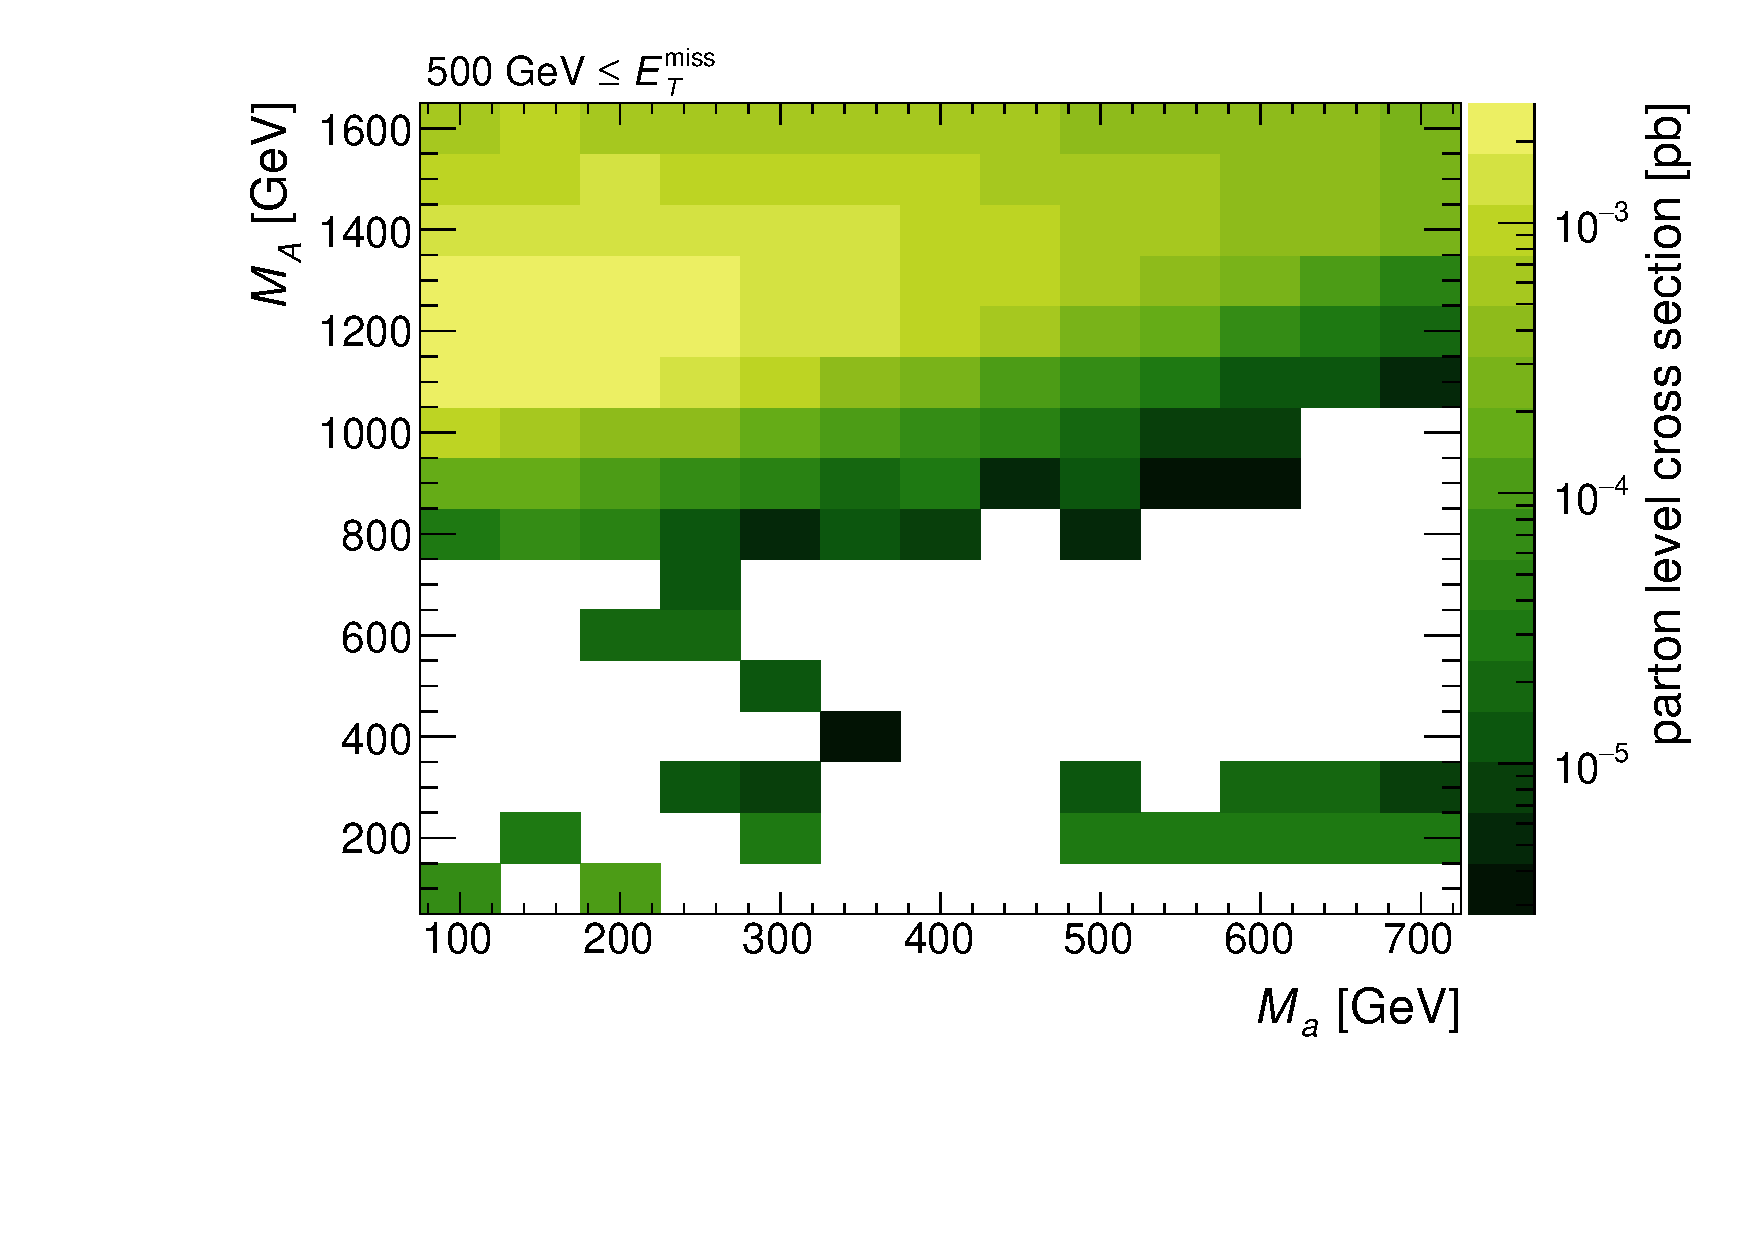
\includegraphics[width = \textwidth]{texinputs/04_grid/figures/monoHbb_parton_level_cross_section_bin_4_ma_vs_mA_lin.pdf}
\end{subfigure}
\caption[$h\rightarrow bb + \MET$ cross-section binned in $\MET$, $\mA$ - $\ma$ plane ]
{
The production cross-section of $h\rightarrow bb + \MET$ signal events at parton level as a function of $(\mA,\ma)$ in each of the four \met bins. 
The remaining parameters take the values
$ \mH=\mHc= \mA, \sinp = 0.35, \tanb = 1, \mDM = 10$ GeV and $ \lap1 = \lap2 = \lam3 = 3 $.
}
\label{fig:monoHbb_xsec_bins_mA_ma}
\end{figure}

\begin{figure}[tbp]
\centering
\begin{subfigure}{0.48\textwidth}
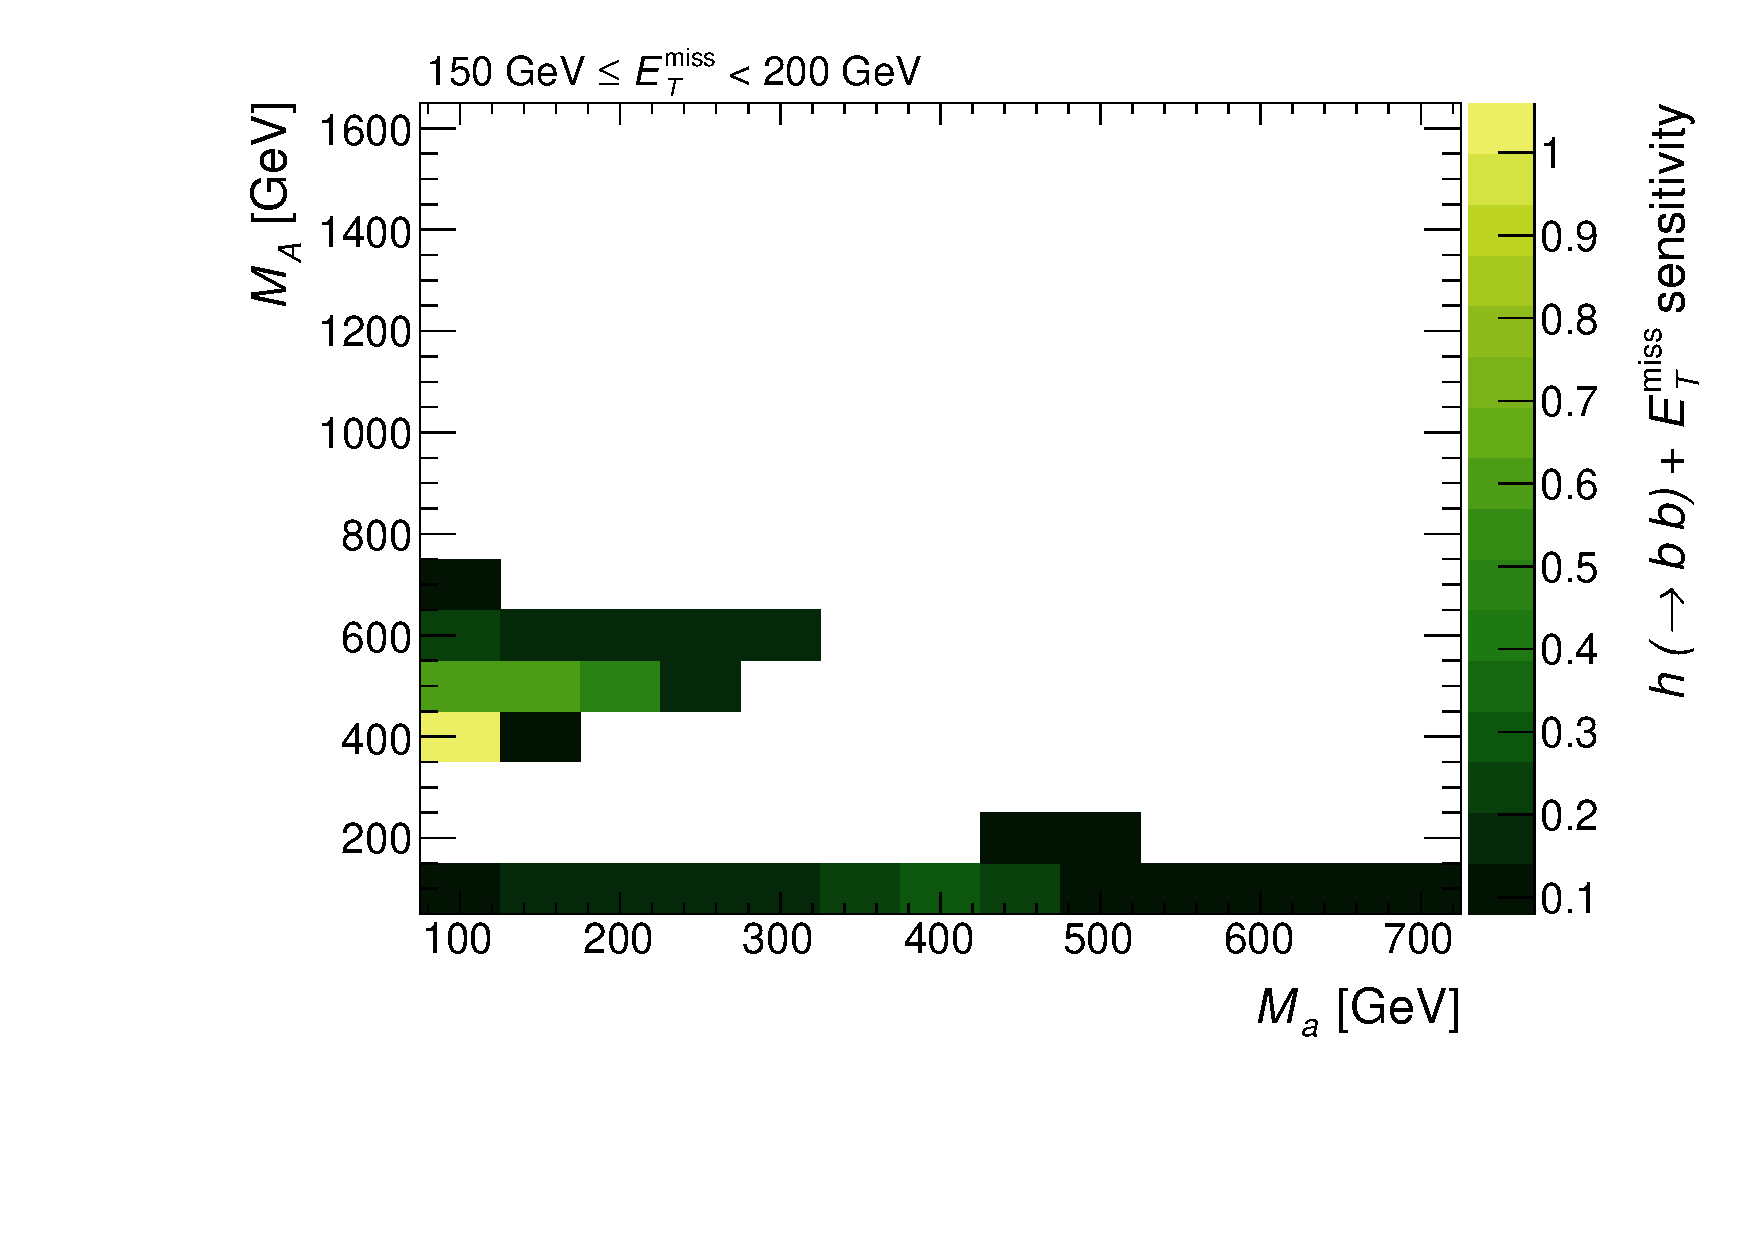
\includegraphics[width = \textwidth]{texinputs/04_grid/figures/monoHbb_sensi_bin_1_ma_vs_mA_lin.pdf}
\end{subfigure}
~
\begin{subfigure}{0.48\textwidth}
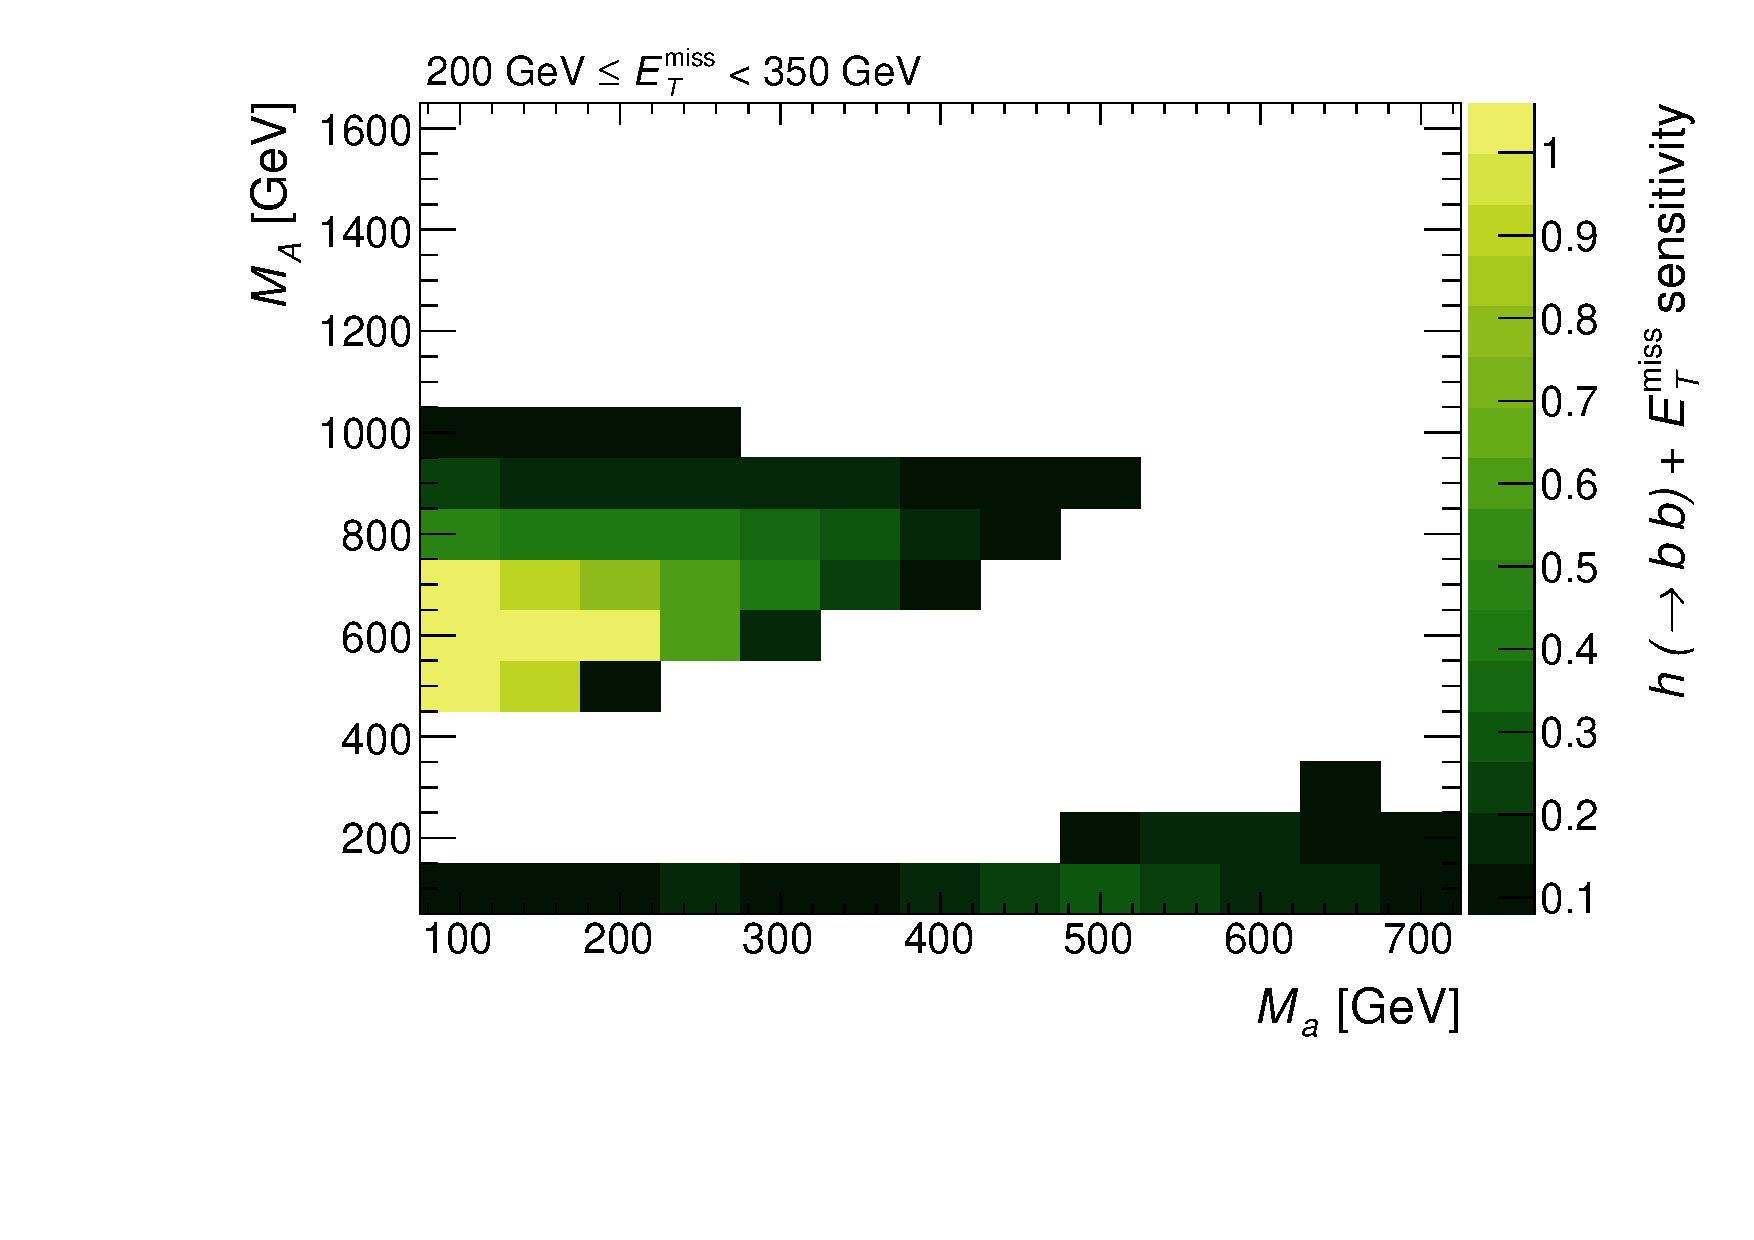
\includegraphics[width = \textwidth]{texinputs/04_grid/figures/monoHbb_sensi_bin_2_ma_vs_mA_lin.pdf}
\end{subfigure}
\\
\centering
\begin{subfigure}{0.48\textwidth}
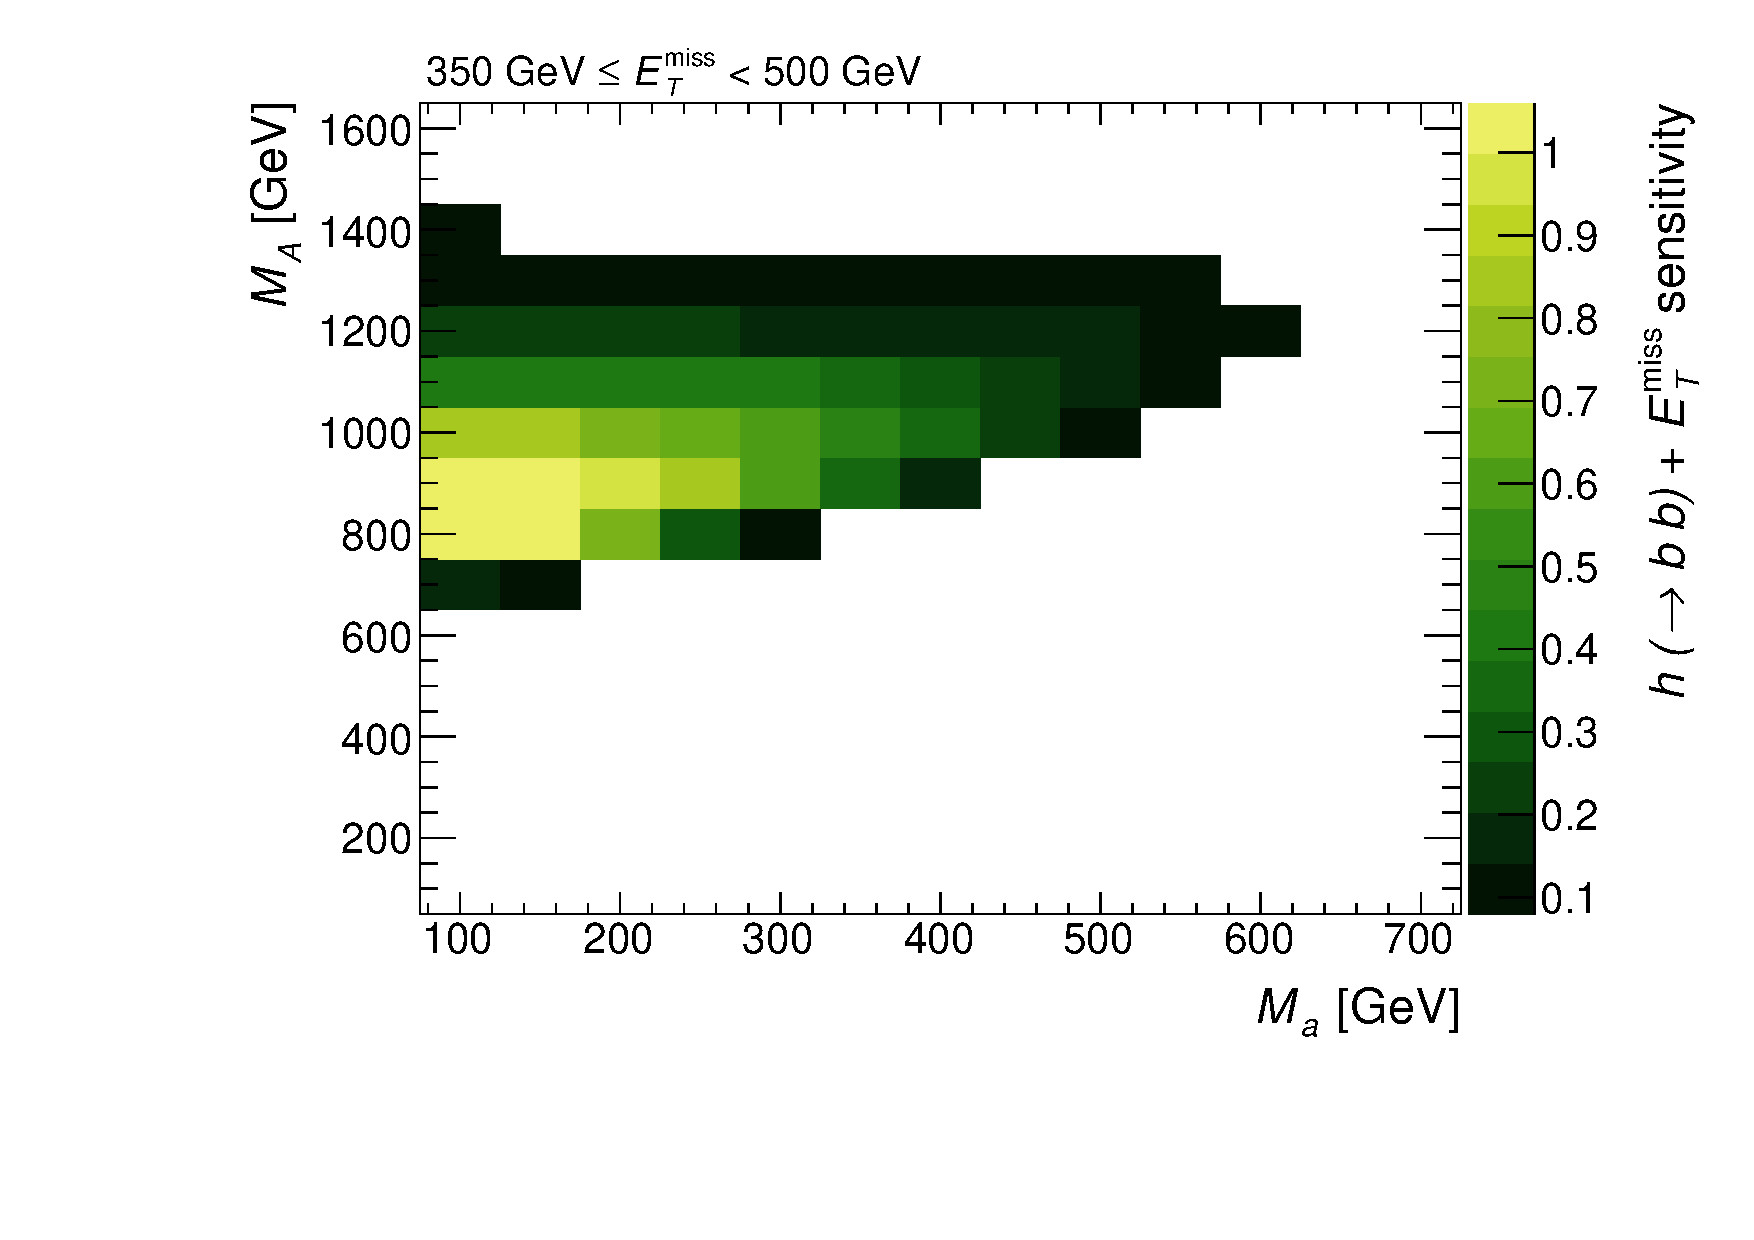
\includegraphics[width = \textwidth]{texinputs/04_grid/figures/monoHbb_sensi_bin_3_ma_vs_mA_lin.pdf}
\end{subfigure}
~
\begin{subfigure}{0.48\textwidth}
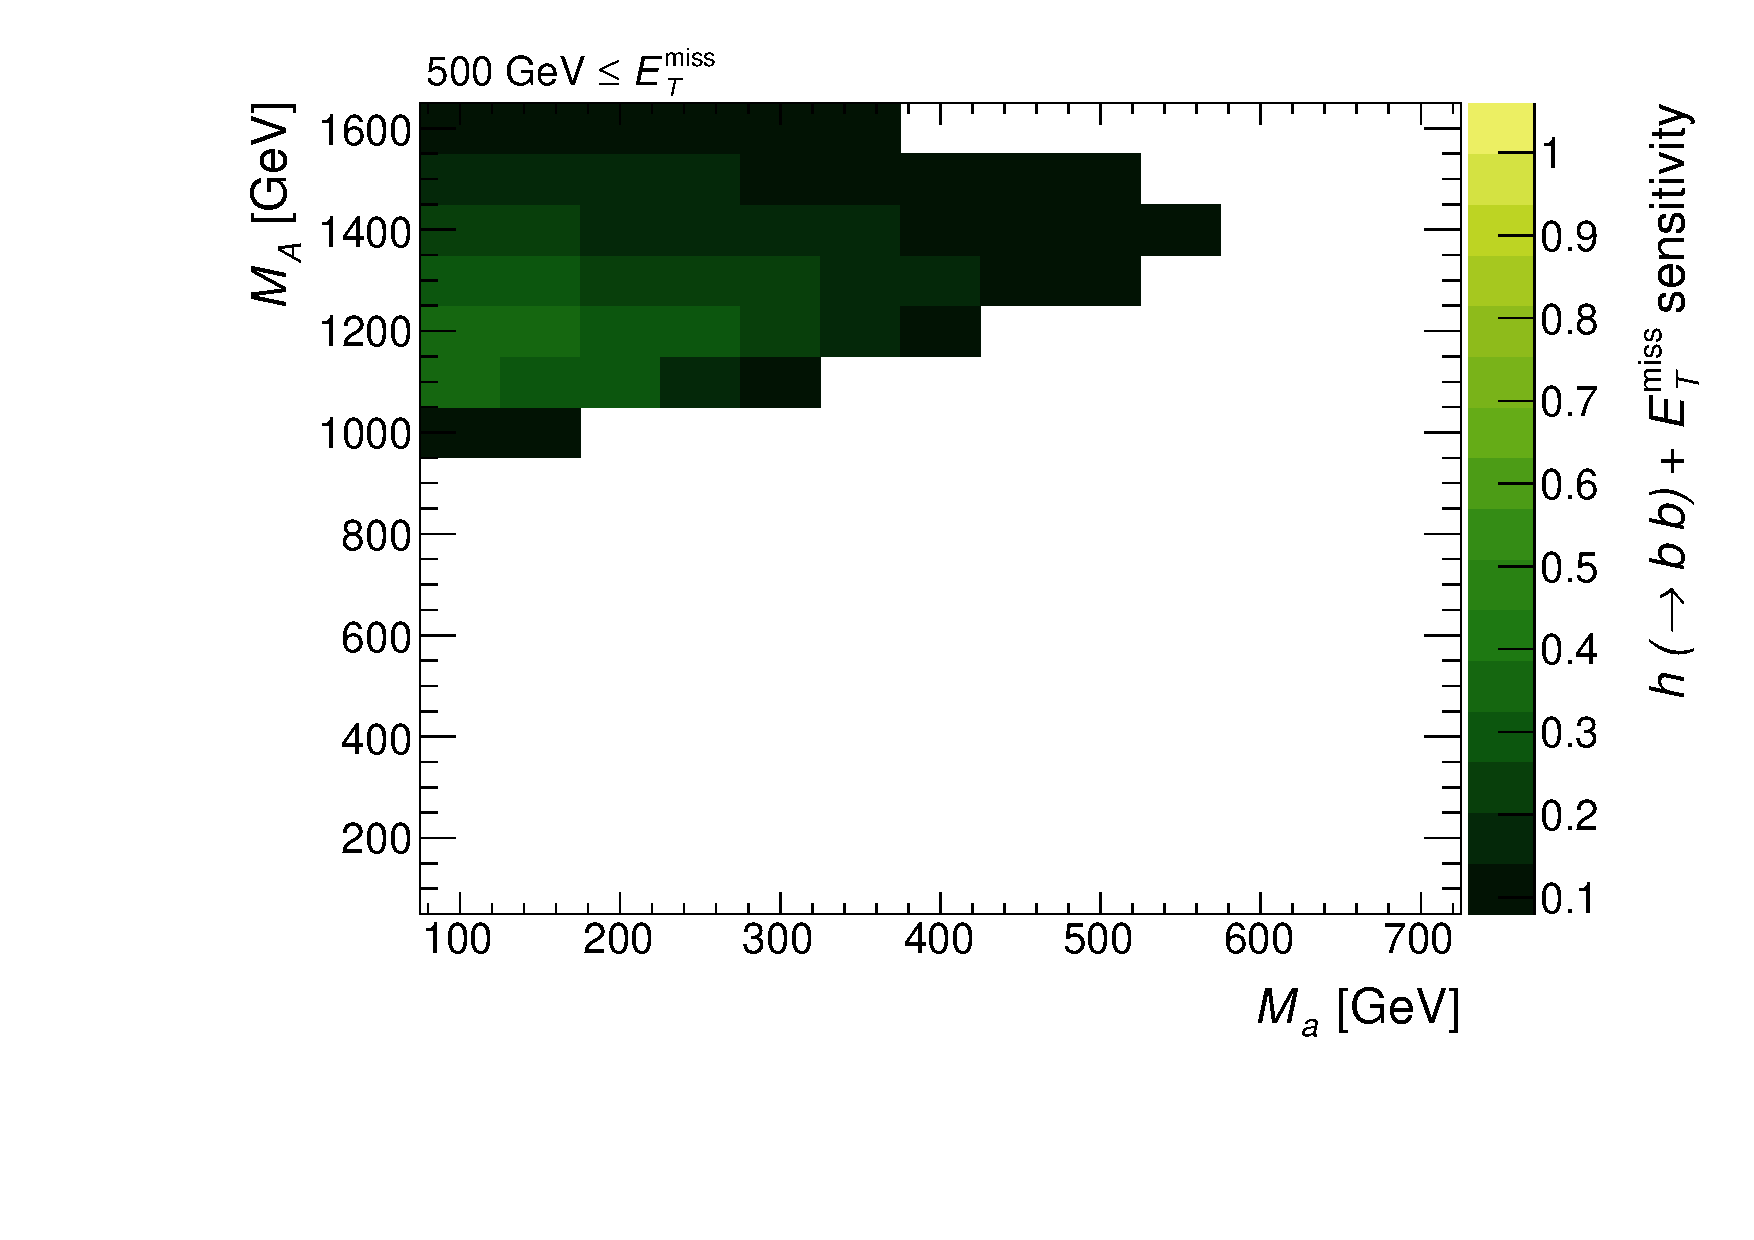
\includegraphics[width = \textwidth]{texinputs/04_grid/figures/monoHbb_sensi_bin_4_ma_vs_mA_lin.pdf}
\end{subfigure}
\caption[Sensitivity to the $h\rightarrow bb + \MET$ signal by $\MET$ bin, $\mA$ - $\ma$ plane]
{Estimated sensitivity to $h\rightarrow bb + \MET$ events as a function of $(\mA,\ma)$ in each of  the four \met bins. 
The sensitivity, defined in Eq.~\ref{eq:monoHbb_sensi}, is based on the limits with reduced model dependence from Ref.~\cite{Aaboud:2017yqz}. 
The remaining parameters take the values
$ \mH=\mHc= \mA, \sinp = 0.35, \tanb = 1, \mDM = 10$ GeV and $ \lap1 = \lap2 = \lam3 = 3 $.}
\label{fig:monoHbb_sensi_bins_mA_ma}
\end{figure}

\begin{figure}[tbp]
\centering
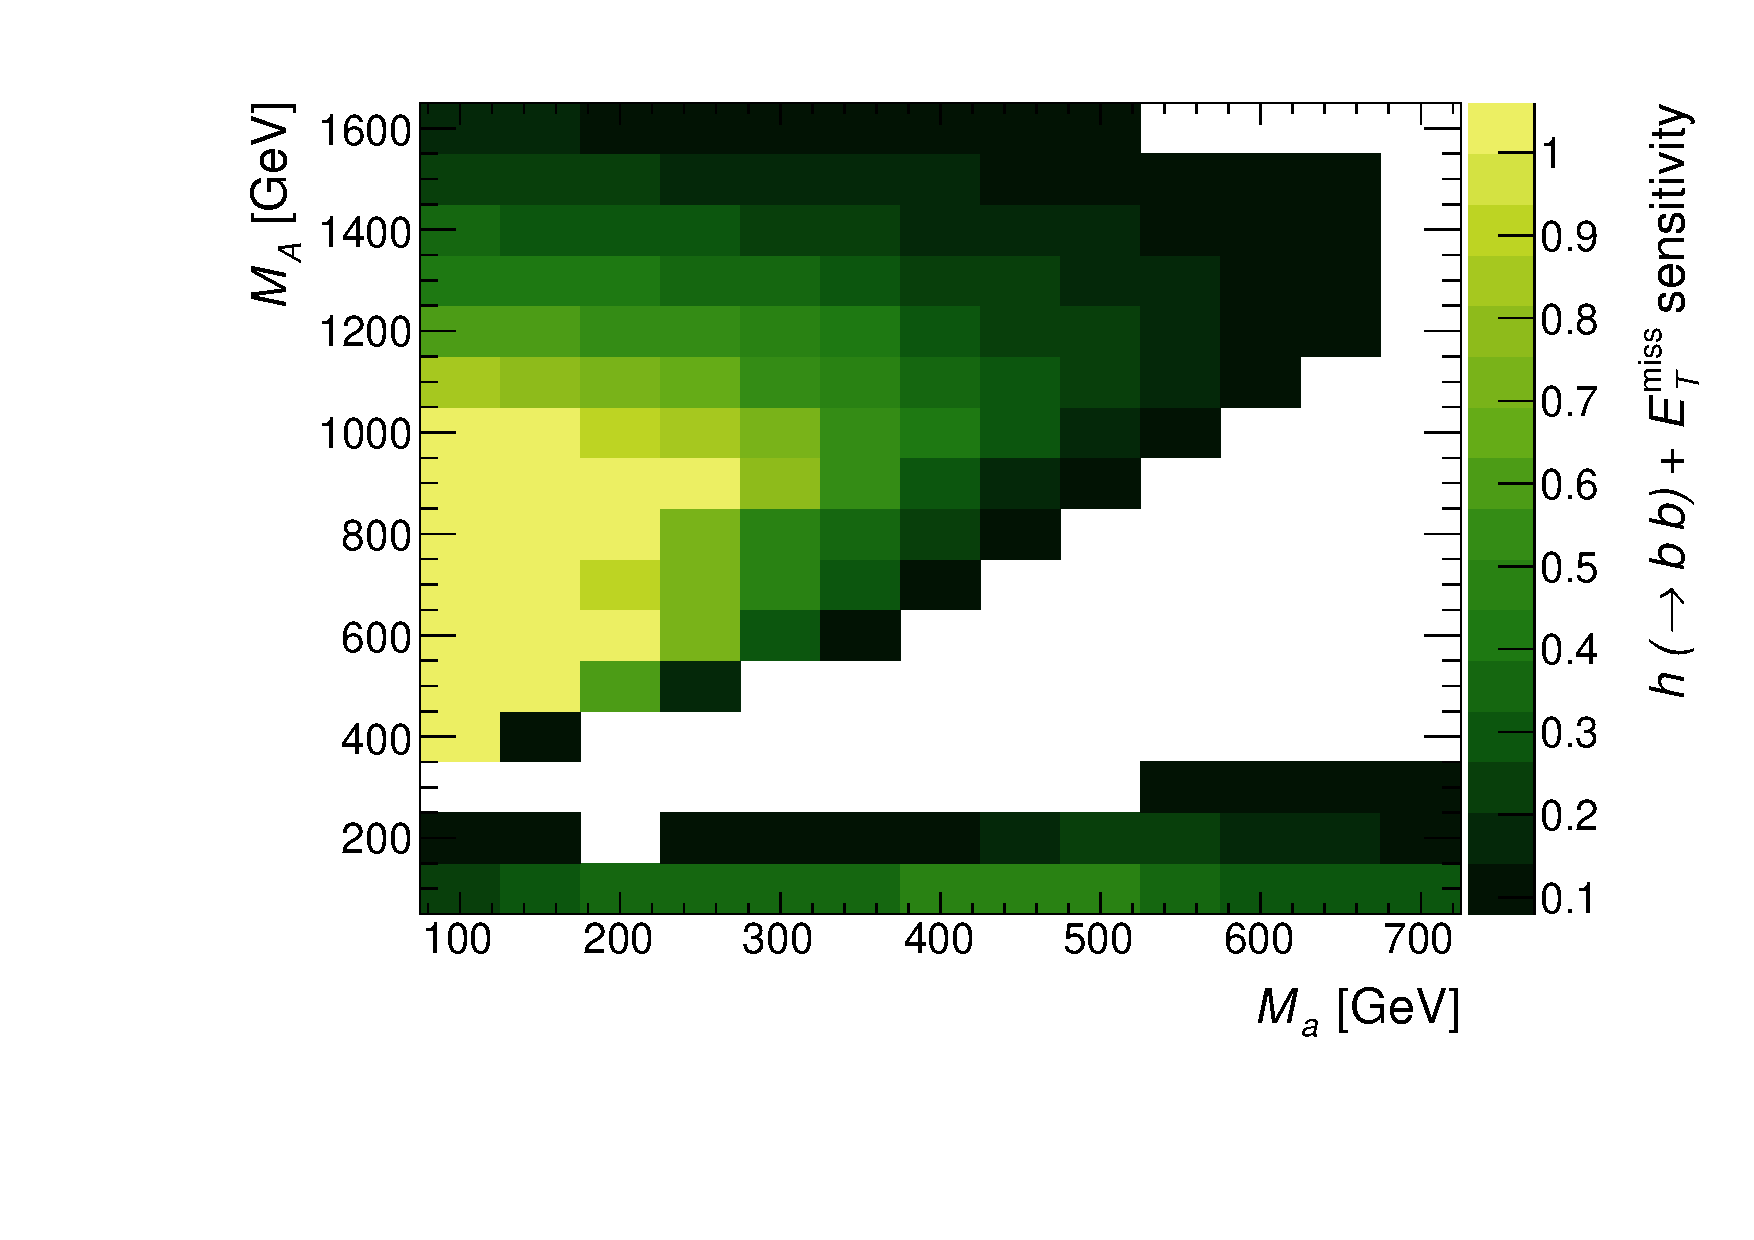
\includegraphics[width=\textwidth]{texinputs/04_grid/figures/monoHbb_sensi_sum_bins_1_2_3_4_ma_vs_mA_lin.pdf}
\caption[Sensitivity to $h\rightarrow bb + \MET$ signals in $\mA$ - $\ma$ plane, summed across $\MET$ bins]
{
Sum over all $\MET$-bins of the estimated sensitivity to $h\rightarrow bb + \MET$ events as a function of $(\mA,\ma)$. 
The sensitivity, defined in Eq.~\ref{eq:monoHbb_sensi}, is based on the limits with reduced model dependence from Ref.~\cite{Aaboud:2017yqz}. 
The remaining parameters take the values $ \mH=\mHc= \mA, \sinp = 0.35, \tanb = 1, \mDM = 10$ GeV and $ \lap1 = \lap2 = \lam3 = 3 $.}
\label{fig:monoHbb_sensi_full_mA_ma}
\end{figure}

\begin{figure}[tbp]
\centering
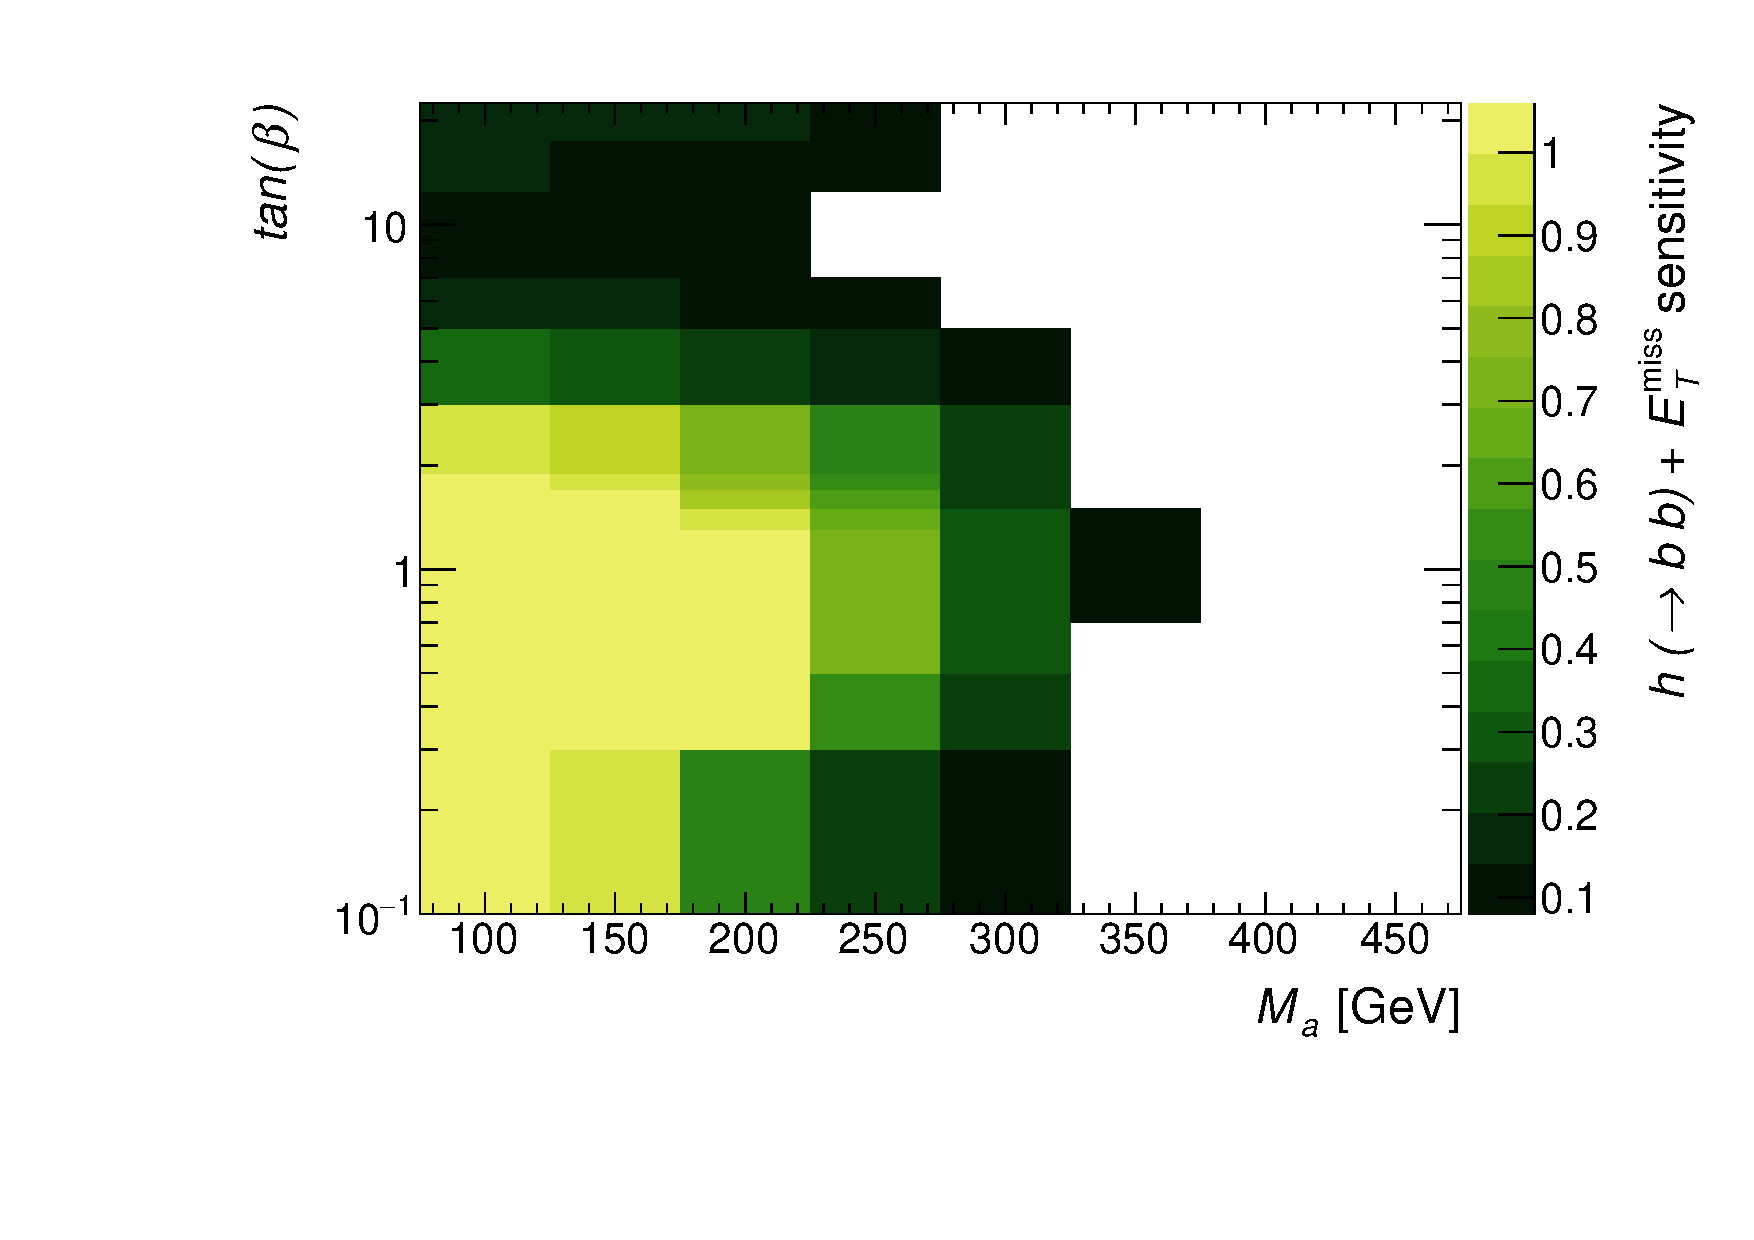
\includegraphics[width=\textwidth]{texinputs/04_grid/figures/monoHbb_sensi_sum_bins_1_2_3_4_ma_vs_tanb_lin.pdf}
\caption[Sensitivity to $h\rightarrow bb + \MET$ signals in $\mA$ - $\tanb$ plane, summed across $\MET$ bins]
{
Sum over all $\MET$-bins of the estimated signal sensitivity to $h\rightarrow bb + \MET$ events as a function of $(\ma,\tanb)$. The sensitivity, defined in Eq.~\ref{eq:monoHbb_sensi}, is based on the limits with reduced model dependence from Ref.~\cite{Aaboud:2017yqz}. The remaining parameters take the values
$ \mH=\mHc=\mA = 600$ GeV, $ \sinp = 0.35, \mDM = 10$ GeV and $ \lap1 = \lap2 = \lam3 = 3 $.}
\label{fig:monoHbb_sensi_full_ma_tanb}
\end{figure}

\begin{figure}[tbp]
\centering
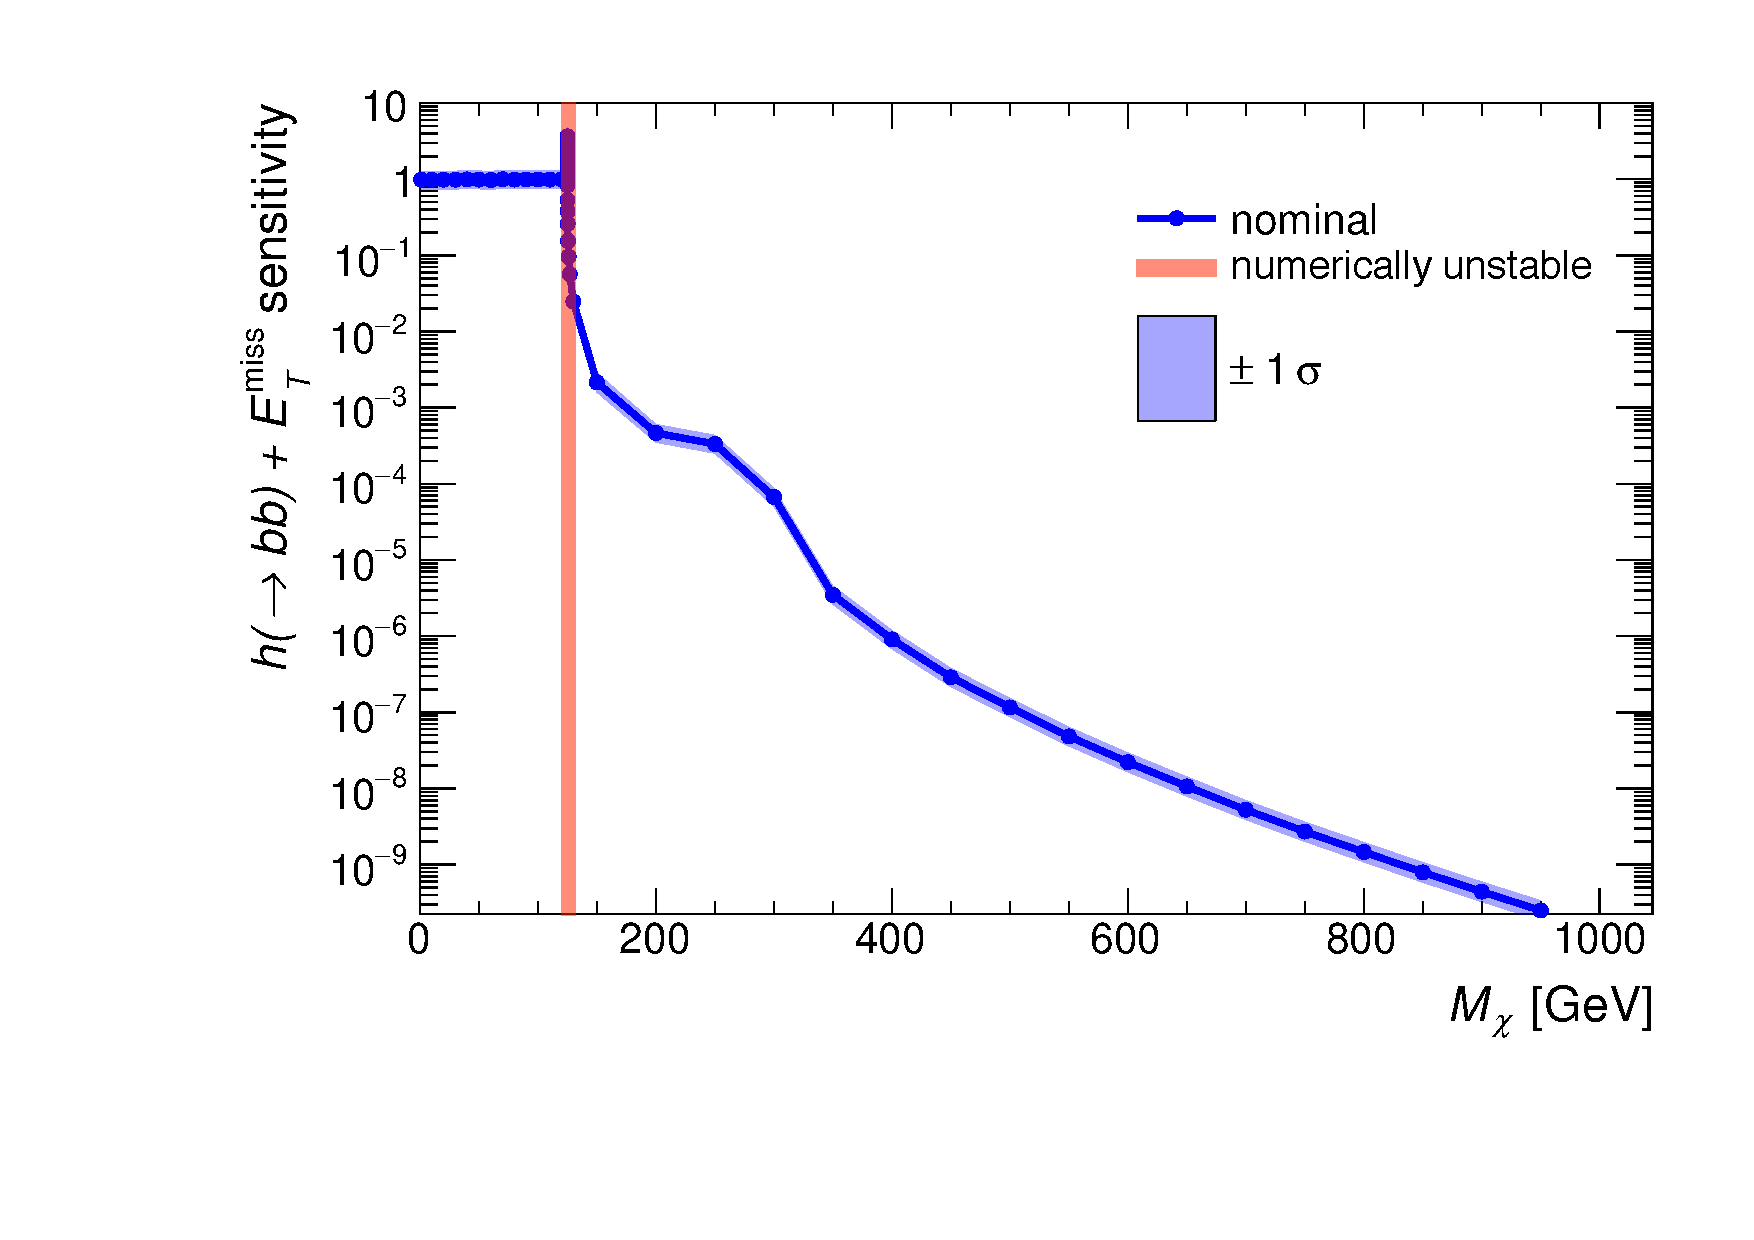
\includegraphics[width=\textwidth]{texinputs/04_grid/figures/monoHbb_sensi_mDM_scan.pdf}
\caption[Sensitivity to $h\rightarrow bb + \MET$ signals with different $\mDM$, summed across $\MET$ bins]
{
Sum over all $\MET$-bins of the estimated signal sensitivity to $h\rightarrow bb + \MET$ events as a function of the Dark Matter mass $\mDM$. 
The sensitivity, defined in Eq.~\ref{eq:monoHbb_sensi}, as well as the uncertainty on the sensitivity (shaded blue)
are based on the limits with reduced model dependence from Ref.~\cite{Aaboud:2017yqz} and the uncertainties described therein. 
The remaining parameters take the values
$ \ma = 250 $ GeV$, \mH=\mHc=\mA = 600$ GeV, $ \sinp = 0.35, \tanb = 1,$ and $ \lap1 = \lap2 = \lam3 = 3 $. 
The sensitivity is constant below $\mDM < \ma/2$, and rapidly drops for $\mDM > \ma/2$. The sensitivity is enhanced for $\mDM = \ma/2$.}
\label{fig:monoHbb_sensi_full_mDM}
\end{figure}

\begin{figure}[tbp]
\centering
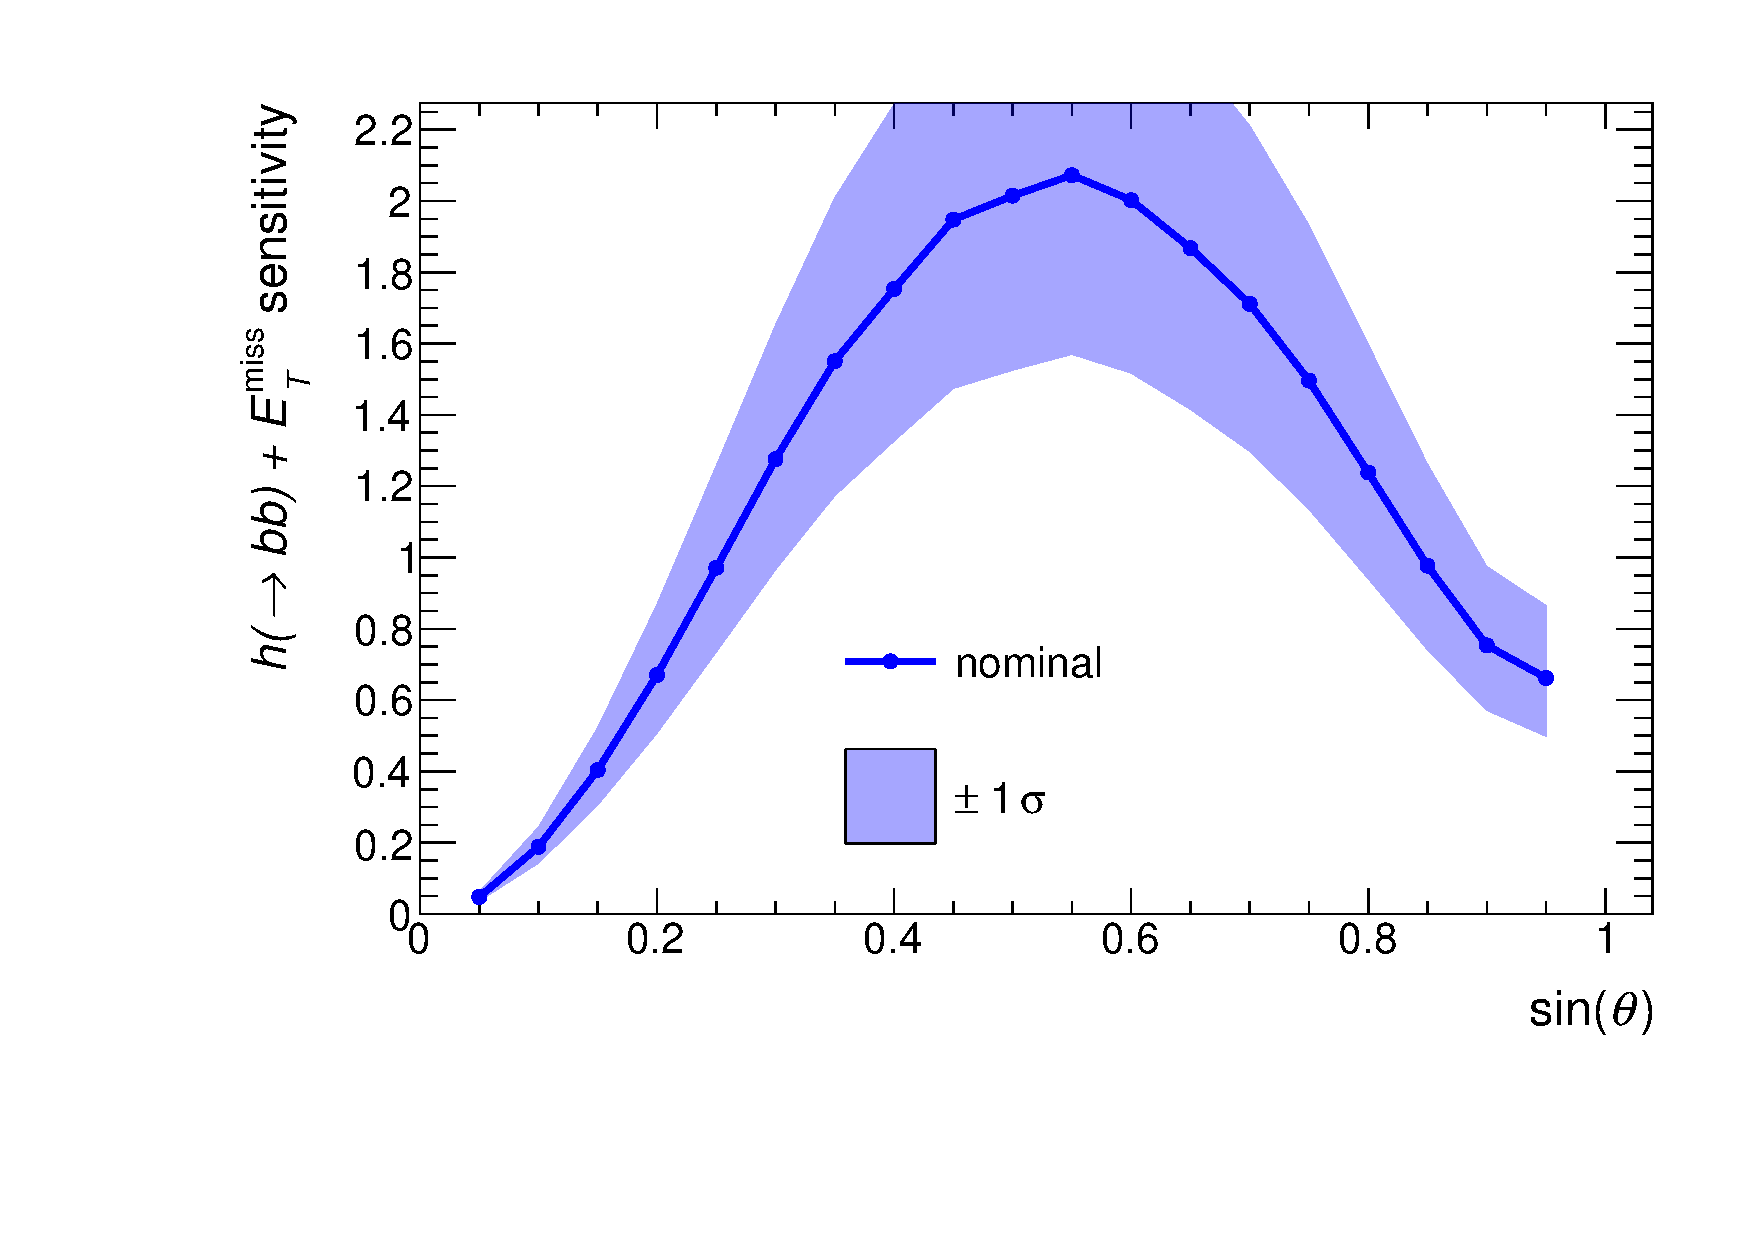
\includegraphics[width=\textwidth]{texinputs/04_grid/figures/monoHbb_sinp_scan_1_sensi_1D.pdf}
\caption[Sensitivity to $h\rightarrow bb + \MET$ signals with different $\sinp$, summed across $\MET$ bins]
{
Sum over all $\MET$-bins of the estimated signal sensitivity to $h\rightarrow bb + \MET$ events as a function of the pseudoscalar mixing parameter $\sinp$. 
The sensitivity, defined in Eq.~\ref{eq:monoHbb_sensi}, as well as the uncertainty on the sensitivity (shaded blue) 
 are based on the limits with reduced model dependence from Ref.~\cite{Aaboud:2017yqz} and the uncertainties described therein. 
The remaining parameters take the values
$ \ma = 200 $ GeV$, \mH=\mHc=\mA = 600$ GeV, $\mDM = 10 $ GeV$, \tanb = 1,$ and $ \lap1 = \lap2 = \lam3 = 3 $.}
\label{fig:monoHbb_sensi_full_sinp_1}
\end{figure}

\begin{figure}[tbp]
\centering
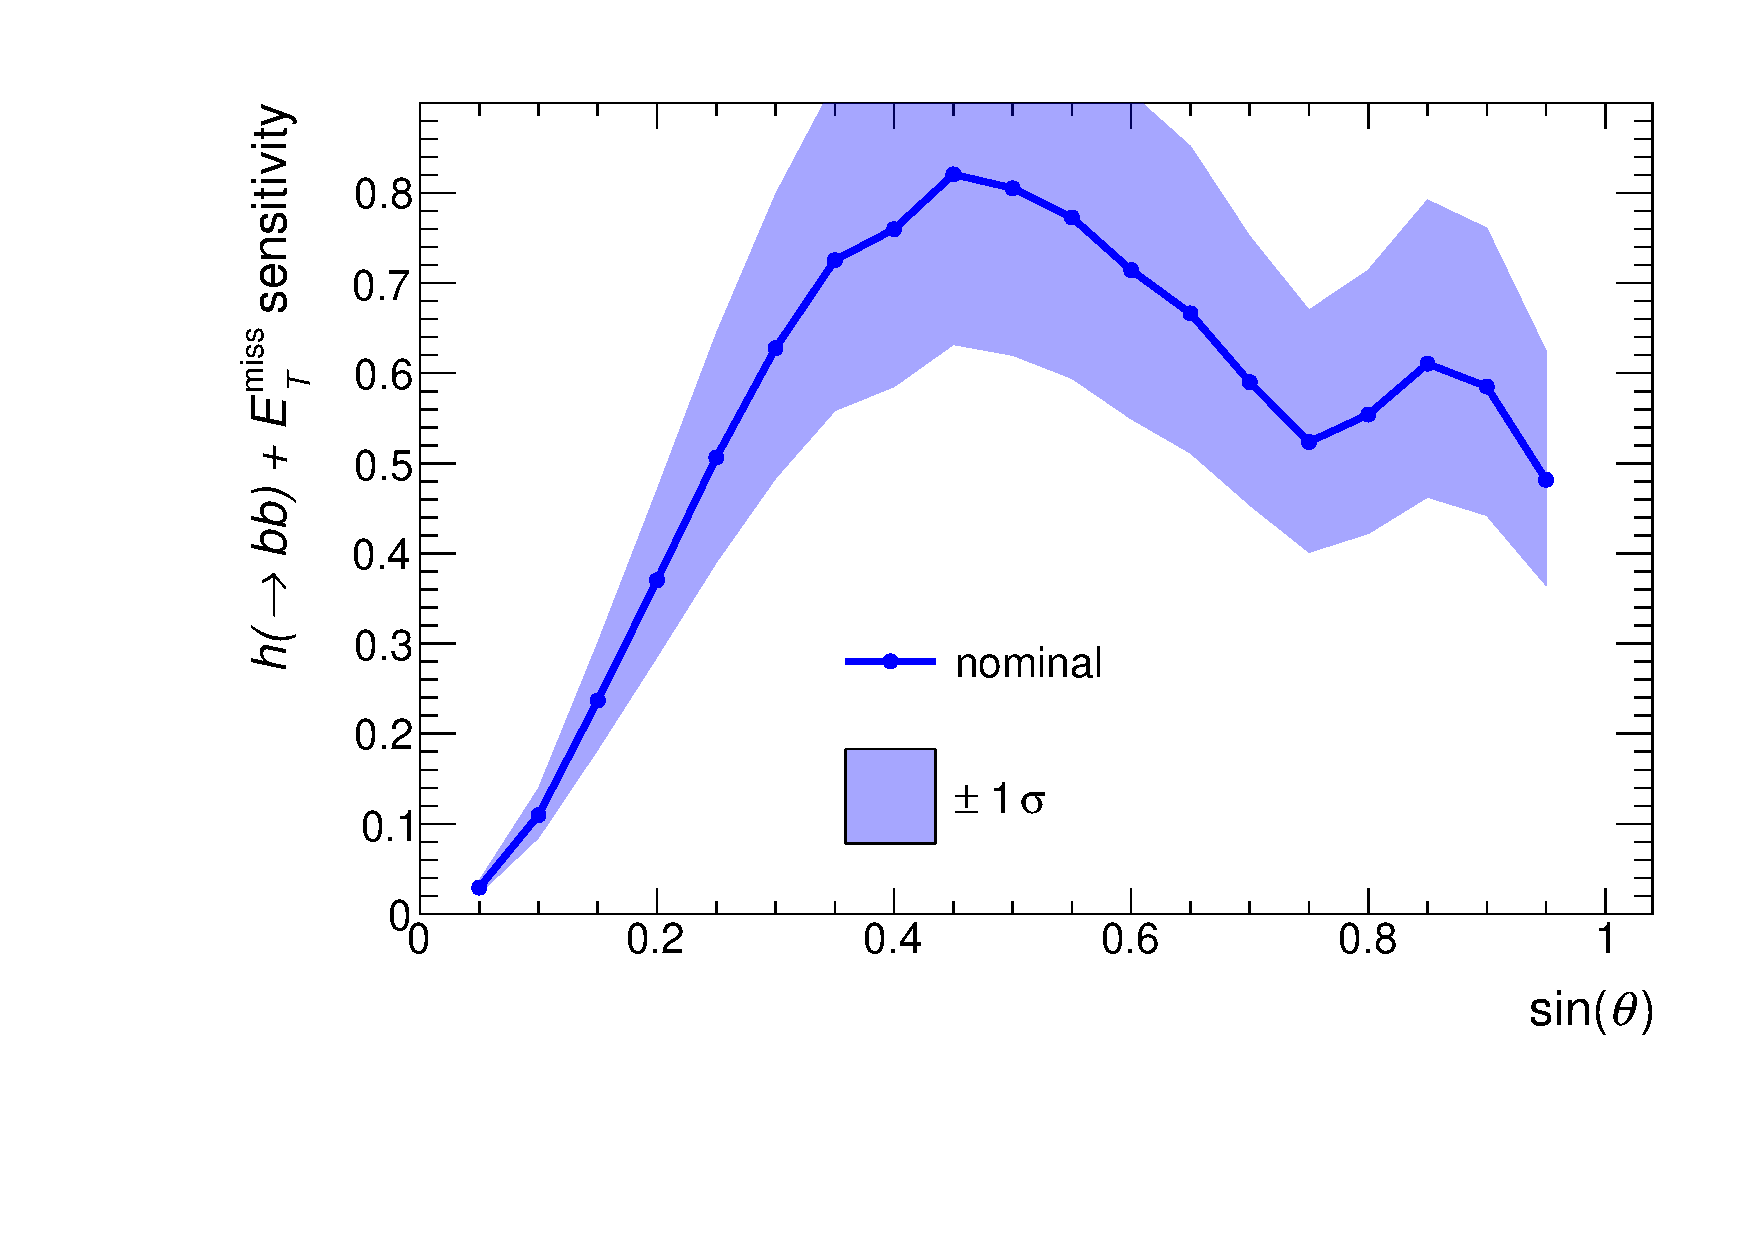
\includegraphics[width=\textwidth]{texinputs/04_grid/figures/monoHbb_sinp_scan_2_sensi_1D.pdf}
\caption[Sensitivity to $h\rightarrow bb + \MET$ signals with different $\sinp$, summed across $\MET$ bins]
{
Sum over all $\MET$-bins of the estimated signal sensitivity to $h\rightarrow bb + \MET$ events as a function of the pseudoscalar mixing parameter $\sinp$. 
The sensitivity, defined in Eq.~\ref{eq:monoHbb_sensi}, as well as the uncertainty on the sensitivity (shaded blue) 
 are based on the limits with reduced model dependence from Ref.~\cite{Aaboud:2017yqz} and the uncertainties described therein. 
The remaining parameters take the values
$ \ma = 350 $ GeV$, \mH=\mHc=\mA = 1000$ GeV, $\mDM = 10 $ GeV$, \tanb = 1,$ and $ \lap1 = \lap2 = \lam3 = 3 $.}
\label{fig:monoHbb_sensi_full_sinp_2}
\end{figure}

The sensitivity of the search  for \monohbb described in \cite{Aaboud:2017yqz} to the 2HDM with pseudoscalar Dark Matter mediator is estimated based on the 
limits with minimal model dependence from \cite{Aaboud:2017yqz}. 
This allows one to directly use parton-level simulations of the 2HDM with pseudoscalar Dark Matter mediator as inputs for the estimate.
Since there is no need to simulate the detector response, which is very costly in terms of CPU-time, the sensitivity can be estimated quickly.
In this way,  more iterations on different versions of the signal grid can be performed.

The limits with minimal model dependence are given in \cite{Aaboud:2017yqz} in terms of the visible cross-section of $\monohbb$ events. 
To compare these values to the parton level simulation results, 
an estimate of the detector efficiency as well as the acceptance of the event selections of the analysis is needed.
This estimate  is provided in \cite{Aaboud:2017yqz} in terms of a single acceptance times efficiency ($\mathcal{A\times\epsilon}$) value per $\MET$ bin. 
The value of $\mathcal{A\times\epsilon}$ corresponds to the probability
 that an event generated at parton level in a given $\MET$ bin is reconstructed in that same $\MET$ bin and passes all selections.
The limits with minimal model dependence are provided separately for each of the four $\MET$ bins used in \cite{Aaboud:2017yqz}.
Thus, the simulated events are binned into those bins (\autoref{fig:monoHbb_xsec_bins_mA_ma}).
Then the simulated cross-section in one $\MET$ bin is compared to the 
limit with minimal model dependence in that $\MET$ bin (\autoref{fig:monoHbb_sensi_bins_mA_ma}). 
In this way, one gets four separate sensitivity estimates.
To obtain a single number estimating the sensitivity of a search that uses all four $\MET$ bins, 
the individual contributions are summed\footnote{This implies that there could be models where the sensitivity in every bin is $<1$, yet the sum is $>1$. 
This is desired for the purpose of estimating sensitivity when designing the grid to be used in a dedicated search, 
since one expects that the full search will be able to exclude those models. 
But for actually excluding models based on the limits with minimal model dependence, the sum is not appropriate.
A better choice for the purpose of exclusion is e.g. the sensitivity of the most sensitive bin.} (\autoref{fig:monoHbb_sensi_full_mA_ma}).
Thus the sensitivity is estimated as
\begin{align}
\label{eq:monoHbb_sensi}
\begin{split}
S^{m} & =  \sum^{\MET\mathrm{-bins}}_{i} S_{i}^{m} \\ & = \sum^{\MET\mathrm{-bins}}_{i} 
\frac{\sigma_{i}^{m,\mathrm{parton}}(h \chi\bar{\chi}) \times \mathcal{BR}_{\mathrm{SM}}(h\rightarrow b\bar{b}) \times [\mathcal{A\times\epsilon}]_{i} }{\sigma_{i}^{\mathrm{observed}}(\monohbb)} ,
\end{split}
\end{align}
where $m$ is a particular model, $i$ is a particular $\MET$ bin, 
$S_{i}^{m}$ the sensitivity to model $m$ based on $\MET$-bin $i$ (\autoref{fig:monoHbb_sensi_bins_mA_ma} ), 
$\sigma_{i}^{m,\mathrm{parton}}(h \chi\bar{\chi})$ the parton level $h\chi\bar{\chi}$ production cross-section 
in bin $i$  predicted by model $m$ (\autoref{fig:monoHbb_xsec_bins_mA_ma}),
$\mathcal{BR}_{\mathrm{SM}}(h\rightarrow b\bar{b})$ the $h\rightarrow b\bar{b}$ branching ratio predicted by the standard model for $M_h = 125$ GeV, 
$[A\times\epsilon]_{i}$ the acceptance times efficiency in bin $i$ as given in \cite{Aaboud:2017yqz},
and $\sigma_{i}^{\mathrm{observed}}(\monohbb)$ the limit on the $\monohbb$ cross-section observed in \cite{Aaboud:2017yqz} in $\MET$ bin $i$.

The $\monohbb$ sensitivity in the sense of eq. \ref{eq:monoHbb_sensi} to a scan in the $(\ma,\mA)$ plane is shown in  \autoref{fig:monoHbb_sensi_bins_mA_ma}.
The sensitivity drops with increasing $\mA = \mH = \mHc$ for $\mA \geq 1 $ TeV because the fraction of resonant signal events drops. 
The drop in the fraction of resonant signal events is caused by increasingly large $\Gamma_A$, 
which allows an increasing fraction of non-resonant signal events, driven by events with very off-shell $A$. % ref ggF-> A -> ah feynman graph
Non-resonant signal events have soft $\MET$ and thus the search is less sensitive to them, since the minimum accepted $\MET$ is $\MET \geq 150$ GeV.
Near the mass diagonal $\ma = \mA$, there is little to no sensitivity. 
This is because the Jacobian peak is at soft $\MET$ for a low mass-splitting $\mA - \ma$
(\autoref{eq:monoH_peak_met}, \autoref{fig:monoHbb_mA_scan_met}, and \autoref{fig:monoHbb_ma_scan_met}).
Furthermore the coupling $g_Aah$ is small when all Higgs bosons are nearly mass degenerate \cite{Bauer:2017ota}, %ref to eq.in theory part(?)
giving a small total cross-section, and lowering the sensitivity even further.
The sensitivity above the mass diagonal ($\mA > \ma$) is larger than the sensitivity below the mass diagonal ($\mA < \ma$).
Two parameter choices cause this asymmetry:
\begin{enumerate}
\item $\mA = \mH = \mHc$, i.e. the neutral and charged CP-even scalars have low masses below the diagonal, but high masses above it, introducing asymmetry.
In \autoref{fig:monoHbb_mH_scan_met} one can see that values of  $\mH = \mHc$ below the mass of the higher-mass pseudoscalar 
give a reduced overall cross-section and a lower fraction of resonant signal events. Both effects reduce sensitivity.
\item $\sinp = 0.35 \neq 1/\sqrt{2}$, i.e. the pseudoscalar mixing is asymmetric. 
$A$ couples comparatively more strongly to SM particles than $a$, and vice versa for the  couplings to the Dark Matter fermion $\chi$.
So the situation below the diagonal corresponds to the case of $\sinp = \sqrt{1-0.35^2} \approx 0.938$ and $\mA > \ma$. 
As can be seen in \autoref{fig:monoHbb_sinp_1_scan_met} and \autoref{fig:monoHbb_sinp_2_scan_met} %update once Eiko/Benedikt add plots
this configuration has a larger fraction of  soft, nonresonant signal events, and correspondingly lower sensitivity 
(\autoref{fig:monoHbb_sensi_full_sinp_1} and \autoref{fig:monoHbb_sensi_full_sinp_2}).
\end{enumerate}

For a scan in $(\ma,\tanb)$ the sensitivity is shown in  \autoref{fig:monoHbb_sensi_full_ma_tanb}. 
At very low $\tanb$, the yukawa coupling to top quarks is large, and most of the signal events come from non-resonant processes. % ref to tanb met scan
The non-resonant processes give soft $\MET$, which lowers the signal acceptance and reduces the sensitivity of the search.
For higher $\tanb$ the fraction of resonant events increases, due to the reduced top Yukawa coupling, increasing the sensitivity.
However reducing the top yukawa coupling also reduces the overall production cross-section. 
This effect is sub-dominant below $\tanb \approx 1.2$, and the sensitivity increases with $\tanb$. 
But above $\tanb \approx 1.2$, the sensitivity loss due to reduced cross-section outpaces the sensitivity gain due to a more resonant signal.
Therefore, above $\tanb \approx 1.2$, the search gets less sensitive with higher $\tanb$.
At very high $\tanb$ ($\geq 10$), this trend is reversed again, as the $\tanb$ enhancement\footnote{we are considering a Yukawa sector of type II} of the 
coupling to b-quarks relative to top quarks becomes so large that it compensates for the lower b quark Yukawa coupling 
corresponding to the lower $b$-quark mass.
At this point $b\bar{b}$ initiated processes start to dominate the production cross-section and drive the increase in sensitivity.

The sensitivity to models with varying $\sinp$ is shown in Figs. \ref{fig:monoHbb_sensi_full_sinp_1} and \ref{fig:monoHbb_sensi_full_sinp_2}.
The sensitivity is $0$ at $\sinp=0$ and $\sinp=1$, since those values correspond to no mixing, and thus no coupling.
So the sensitivity is in general not monotonous in $\sinp$ (\autoref{fig:monoHbb_sensi_full_sinp_1}).
For intermediate values, $\sinp$ influences the couplings of the pseudoscalars to  Dark Matter, as well as to standard model fermions, 
and also the coupling strength of trilinear scalar vertices such as $g_{Aah}$ \cite{Bauer:2017ota}. 
Increasing the couplings increases the cross-section and thereby the sensitivity.
However, increasing some couplings can also increase $\Gamma_A$ and thereby decrease the resonant fraction of signal events.
This means that there can be more than one local maximum in the sensitivity curve (\autoref{fig:monoHbb_sensi_full_sinp_2}).
The number and location  of maxima and turning points in the sensitivity  depends on the precise interplay of the couplings.
The couplings depend on all other model parameters including all the Higgs masses, 
so tuning the $\sinp$ of a parameter scan to the sensitivity in a single point can lead to sub-optimal sensitivity in other points.

The sensitivity to models with varying $\mDM$ is shown in  \autoref{fig:monoHbb_sensi_full_mDM}.
Above threshold ($\mDM < \ma/2$), the sensitivity stays constant. 
This constant sensitivity results from the constant  signal $\MET$ shape (\autoref{fig:monoHbb_mDM_scan_met}), and the constant signal cross-section.
At threshold ($\mDM = \ma$) the sensitivity is enhanced because the partial width for $ a \rightarrow \chi \bar{\chi} $ is enhanced, 
increasing the signal cross-section.
Below threshold ($\mDM > \ma/2$), the sensitivity drops rapidly. 
The reason for the rapid drop in sensitivity is that $\mDM > \ma/2$ requires a virtual $a^{\star} \rightarrow \chi\bar{\chi}$ decay in the  signal event. 
The rate of this virtual $a$ decay is strongly suppressed by the typically  narrow width of  $a$. 
The width of $a$ is substantially reduced once $a\rightarrow \chi \bar{\chi}$ is kinematically inaccessible, 
as $\Gamma_{a\rightarrow \chi \bar{\chi}}$ is a large contribution to the total width of $a$ for $\mDM \leq \ma/2$ \cite{Bauer:2017ota}.
There is a slight bump in sensitivity for $\mDM \approx \mA/2$, when the $A\rightarrow \chi\bar{\chi}$ hits it's threshold,
but the absolute sensitivity remains negligible.
